\documentclass[12pt,a4paper]{article}
\usepackage[utf8]{inputenc}

\usepackage{amsmath}
\usepackage{amsfonts}
\usepackage{amssymb}
\usepackage{graphicx}
\usepackage{listings}
\usepackage[margin=1.0in]{geometry}
\usepackage{caption}
\usepackage{subcaption}
\usepackage{float}
\usepackage[utf8]{inputenc}
\usepackage{refstyle}
\usepackage{spverbatim}
\usepackage{listings}
\usepackage{csvsimple}
\usepackage{adjustbox}
\usepackage{cancel}
\usepackage{scalerel,stackengine}
\stackMath
\newcommand\reallywidehat[1]{%
\savestack{\tmpbox}{\stretchto{%
  \scaleto{%
    \scalerel*[\widthof{\ensuremath{#1}}]{\kern-.6pt\bigwedge\kern-.6pt}%
    {\rule[-\textheight/2]{1ex}{\textheight}}%WIDTH-LIMITED BIG WEDGE
  }{\textheight}% 
}{0.5ex}}%
\stackon[1pt]{#1}{\tmpbox}%
}
\parskip 1ex

\lstset{numbers=left,
	title=\lstname,
	numberstyle=\tiny, 
	breaklines=true,
	tabsize=4,
	language=Python,
	morekeywords={with,super,as},,
	frame=single,
	basicstyle=\footnotesize\tt,
	commentstyle=\color{comment},
	keywordstyle=\color{keyword},
	stringstyle=\color{string},
	backgroundcolor=\color{background},
	showstringspaces=false,
	numbers=left,
	numbersep=5pt,
	literate=
		{æ}{{\ae}}1
		{å}{{\aa}}1
		{ø}{{\o}}1
		{Æ}{{\AE}}1
		{Å}{{\AA}}1
		{Ø}{{\O}}1
	}

\usepackage{bm}
\usepackage{hyperref}
\usepackage[usenames, dvipsnames]{color}

\begin{document}

\begin{center}
\LARGE{\textbf{Project 1: Classification and Regression, from linear and logistic regression to neural networks}}
\\
\large{\textbf{Course: FYS-STK4155}}
\\
\large{\textbf{Semester: Autumn 2020}}
\\
\large{\textbf{Name: Sander Losnedahl}}
\end{center}

\begin{center}
\Large{\textbf{Abstract}}
\end{center}

\noindent a

\newpage

\begin{center}
\Large{\textbf{Introduction}}
\end{center}

\noindent a

\newpage

\begin{center}
\Large{\textbf{Preliminaries}}
\end{center}

\noindent \textbf{The github page} can be found at \href{{https://github.com/sanderwl/FYS-STK4155}}{\nolinkurl{https://github.com/sanderwl/FYS-STK4155}} under the folder "project 1". Here you can find the python code used to generate the results in this report as well as the report itself with figures and data.
\\
\textbf{Scaling the data} is necessary in order to make sense of the output values. If the data is unscaled, the resulting numbers will not make much sense as we have no reference to what are low and high numbers. When we scale the data we subtract the sample mean and divide by the sample standard deviation of the data, we essentially make the data centred around zero with standard deviation one. This way, we always have a reference to the outcome as it is always relative to zero. Additionally, most regression algorithms rely on the data having lower distance between the data points, making scaling an important pre-processing step.
\\
\textbf{Noise level} is a recurrent theme throughout this report. Noise is added to the data (exercises a-e) in order to prepare for the real data later on. The noise that is added has a standard normal distribution with standard deviation $1$ and maximum value of $1$ at its mean of zero. This noise is then multiplied with a constant ($0.001$ in most cases in this report) in order to adjust the noise level. 
\\
\textbf{The train/test split} will be $75/25$ in this project. When performing regression, we need to train the algorithm using the training set, as well as validate the trained algorithm using the independent test set. There is no set ratio which is considered the best, but the training set should include the majority of the observations. 

\newpage

\begin{center}
\Large{\textbf{Exercise 1a): Stochastic gradient descent}}
\end{center}

\begin{center}
\large{\textbf{The Franke function}}
\end{center}

\noindent a

\begin{center}
\large{\textbf{Concepts of gradient descent and the cost function}}
\end{center}

\noindent In the last project, we utilized least squares solutions on the form $\boldsymbol{\hat{\beta}} = (\textbf{X}^T\textbf{X})^{-1}\textbf{X}^T\hat{y}$ in order to find the regression coefficients yielding the lowest residual sum of squares. However, this method relies on taking an matrix inverse of the data, which often is not feasible. Another approach which does not utilize matrix inversion is gradient descent. This method instead relies on finding the minimum value of some cost function dependent on the regression coefficients. In this exercise, we will use the MSE as the cost function is given by equation \ref{eq:MSEdef}

\begin{equation}\label{eq:MSEdef}
\begin{aligned}
MSE = C(\boldsymbol{\beta}) = \frac{1}{n}\sum_{i = 1}^n (f - \hat{y})^2
\end{aligned}
\end{equation}

\noindent where f is the Franke function we are trying to predict and $\hat{y}$ is the prediction. Like previously mentioned, we want to find where this function has its minimum, as this point will yield the best regression coefficients. Gradient descent does not attempt to find this point directly, but iteratively. We can find the gradient of equation \ref{eq:MSEdef} and iteratively move the values of our regression coefficients along the line of most negative gradient. After a given number of iterations, we are bound to find the minimum of the cost function, or at least a local minimum (this will be discussed later). In order to find the gradient, we can simply take the partial derivative of equation \ref{eq:MSEdef} with respect to each individual regression coefficient

\begin{equation}\label{eq:MSEder}
\begin{aligned}
\frac{\partial C(\boldsymbol{\beta})}{\partial \boldsymbol{\beta}} 
\\
\frac{\partial \frac{1}{n} \sum_{i = 1}^n (f-\hat{y})^2}{\partial \boldsymbol{\beta}} 
\\
\frac{\partial \frac{1}{n} \sum_{i = 1}^n (f-\textbf{X}\boldsymbol{\hat{\beta}})^2}{\partial \boldsymbol{\beta}} 
\\
\frac{2}{n} \sum_{i = 1}^n \textbf{X}(f - \textbf{X}\boldsymbol{\hat{\beta}}) 
\end{aligned}
\end{equation}

\noindent As mentioned, we iteratively follow the direction in which the gradient is most negative. The number of iterations to perform is called the epoch and is usually just set to a very high number. When we are approaching the minimum or a local minimum, the algorithm which only follows the gradient will be "stuck" and wiggle back and fourth around this minimum or local minimum. Therefore, any iterations following the point of becoming "stuck" is useless, so the algorithm should be stopped at this point.
\\
We have so far only discussed in which direction we are to move, but how large steps should we take in that direction? This parameter is called the learning rate and is typically in the between zero and one (around $0.01$). The learning parameter can either be static or adaptive. The former means that we are only moving a set distance every iteration, while the latter means that we are changing the distance we are moving depending on what iterations we are currently on. A adaptive learning rate depends on the schedule which sets the learning rate for each epoch iteration. In this project we use the time based schedule which is given by equation \ref{eq:scheduleTIME}

\begin{equation}\label{eq:scheduleTIME}
\begin{aligned}
\frac{t_0}{t + t_1}
\end{aligned}
\end{equation}

\noindent where $t_0$ and $t_1$ are constants and t is given by epoch iterations $\times$ number of samples. 
\\
The problem with gradient descent is that if we have a very large number of features (polynomial degrees here), the gradient descent algorithm will take a very long time to run. To counter this problem, we introduce a variant of the gradient descent called stochastic gradient descent.

\begin{center}
\large{\textbf{Taking a stochastic approach to gradient descent}}
\end{center}

\noindent The stochastic gradient descent approach relies on simply utilizing a part of the entire data. The part used is called batch or mini-batch and can be just a single observation (actual stochastic gradient descent) or some where in between one and the number of observations (semi-stochastic gradient descent). This technique works as we are iterating over the number of batches as well as the number of epochs, each time taking a random sample from the original observations. Taking only a sample from the observation works because we are repeating the gradient descent process a large number of times equal to $\frac{\textrm{number of observations}}{\textrm{size of batch}}$. Since we are only utilizing one or a few number of observations, equation \ref{eq:MSEder} can be written as

\begin{equation}\label{eq:MSEderSTO}
\begin{aligned}
2 \textbf{X}(f - \textbf{X}\boldsymbol{\hat{\beta}}) 
\end{aligned}
\end{equation}

\noindent and the t in equation \ref{eq:scheduleTIME} will instead be epoch iteration $\times$ number of samples $+$ batch iteration.
\\
So far we have only considered the gradient descent in terms of its least squares equivalent, however, we also want to implement the ridge equivalent. In the Ridge case, the gradient descent concept and algorithm is exactly the same as the OLS case, but the gradient at which we try to find the MSE minimum look slightly different as we need to add a penalty term $\lambda \times \boldsymbol{\hat{\beta}}$ as shown in equation \ref{eq:MSEderSTOridge}

\begin{equation}\label{eq:MSEderSTOridge}
\begin{aligned}
2 \textbf{X}(f - \textbf{X}\boldsymbol{\hat{\beta}}) + \lambda \boldsymbol{\hat{\beta}}
\end{aligned}
\end{equation}

\noindent where the penalty parameter $\lambda$ is typically between zero and one. 

\begin{center}
\large{\textbf{Parameter dependencies for static learning rate}}
\end{center}

\noindent So far we have merely discussed the theoretical concepts of gradient descent, but now we will implement to perform the stochastic gradient descent. We will then vary the different parameters and see how our cost function varies with the different parameters. First, let us set up some standard parameters so we keep the analysis consistent as seen in table \ref{tab:standardParam}

\begin{table}[h]
\caption{\label{tab:standardParam} An overview of standard parameters to be used in the analysis.}
\centering
\begin{tabular}{c|c|c|c|c}
 & static OLS & static Ridge & adaptive OLS & adaptive Ridge\\
\hline
Number of observation n & $100$ & $100$ & $100$ & $100$\\
\hline
Noise-level & $0.001$ & $0.001$ & $0.001$ & $0.001$\\
\hline
Penalty $\lambda$ & None & $0.01$ & None & $0.01$\\
\hline
Model complexity p & $5$ & $5$ & $5$ & $5$\\
\hline
Batch size & $10$ & $10$ & $10$ & $10$\\
\hline
Epoch size & $100$ & $100$ & $100$ & $100$\\
\hline
Initial learning rate & $0.01$ & $0.01$ & $0.01$ & $0.01$\\
\hline
Schedule & None & None & $\frac{t_0}{t+t_1}$ & $\frac{t_0}{t+t_1}$\\
\end{tabular}
\end{table}

\noindent We can now use the values in table \ref{tab:standardParam} as a standard when we want to study the dependence on a single parameter. Let us first study how the MSE varies as function of an increasing number of epoch iterations using our standard parameters with static learning rate

\begin{figure}[H]
\centering
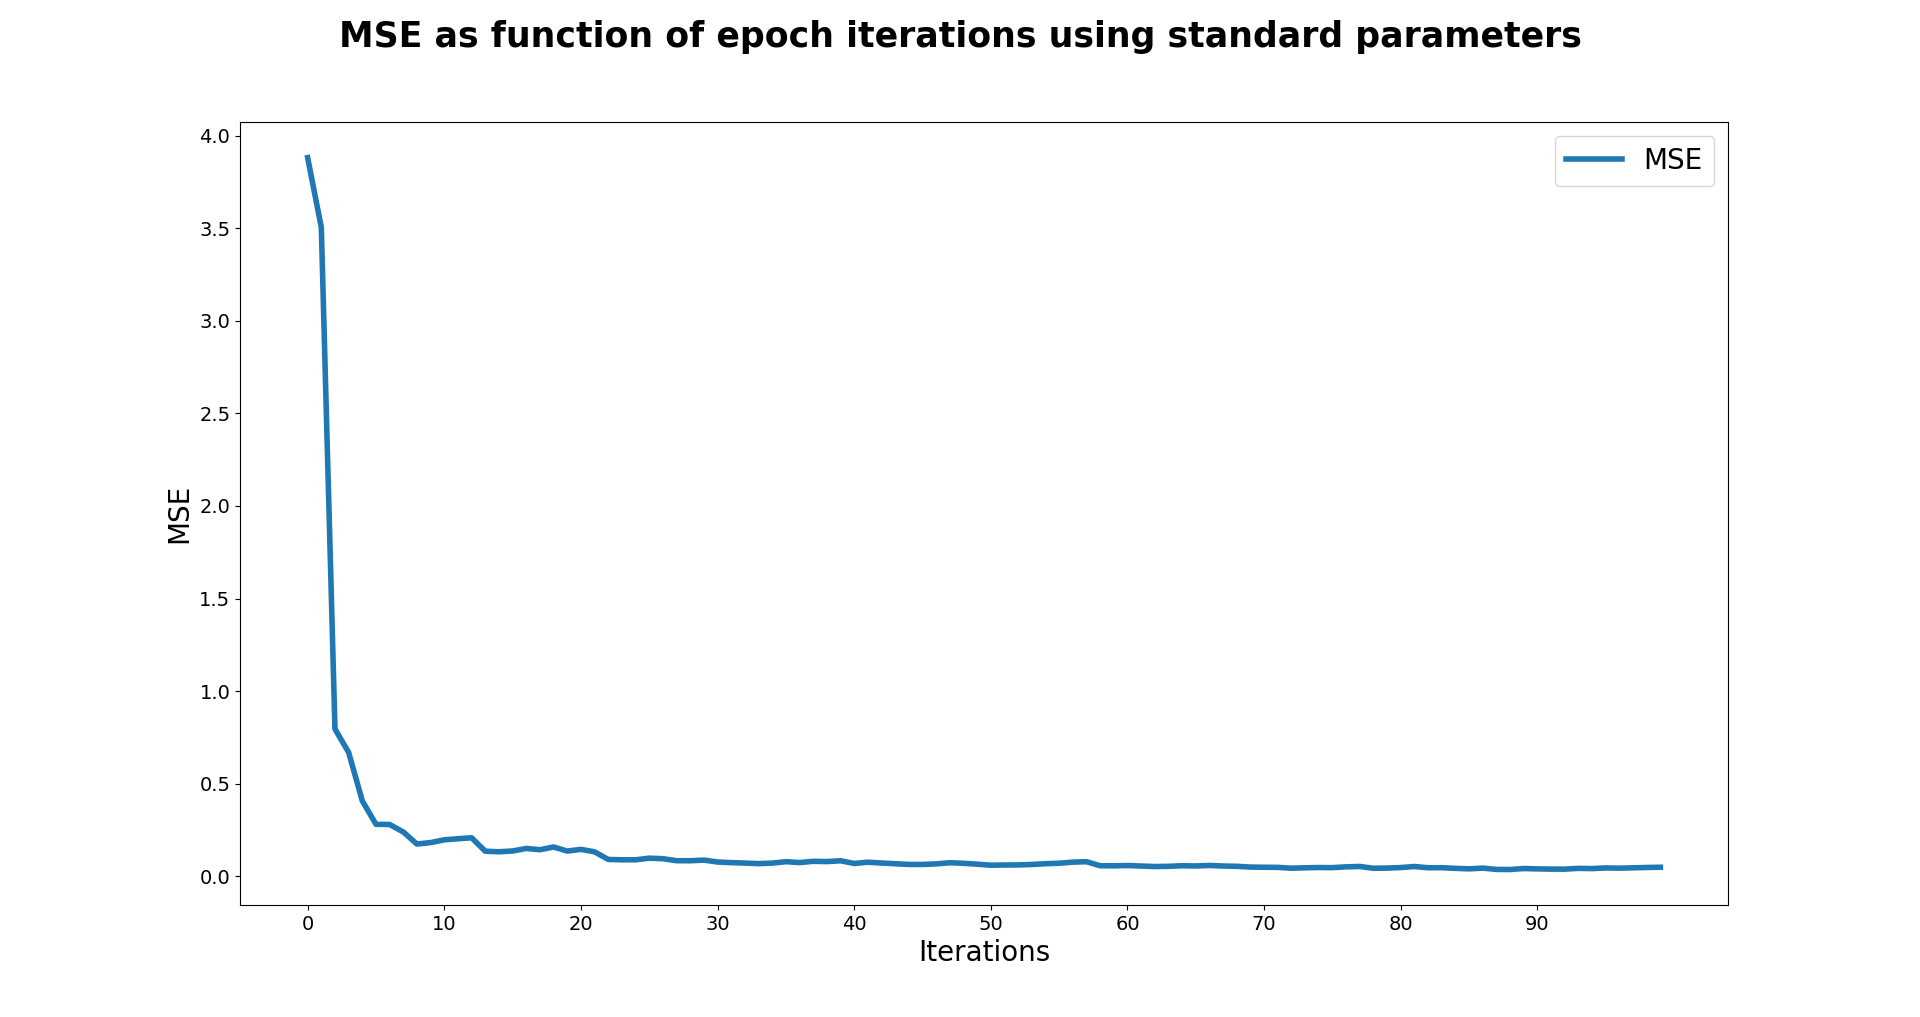
\includegraphics[width = 1\linewidth]{C:/Users/Sander/Documents/GitHub/FYS-STK4155/Project2/Project2/Report/Figures/MSEvsEPOCH_StandardOLS.PNG}
\caption{\label{fig:MSEvsEPOCHstandard} The MSE as function of number of epoch iterations using static learning rate and OLS equivalent SGD.}
\end{figure}

\begin{figure}[H]
\centering
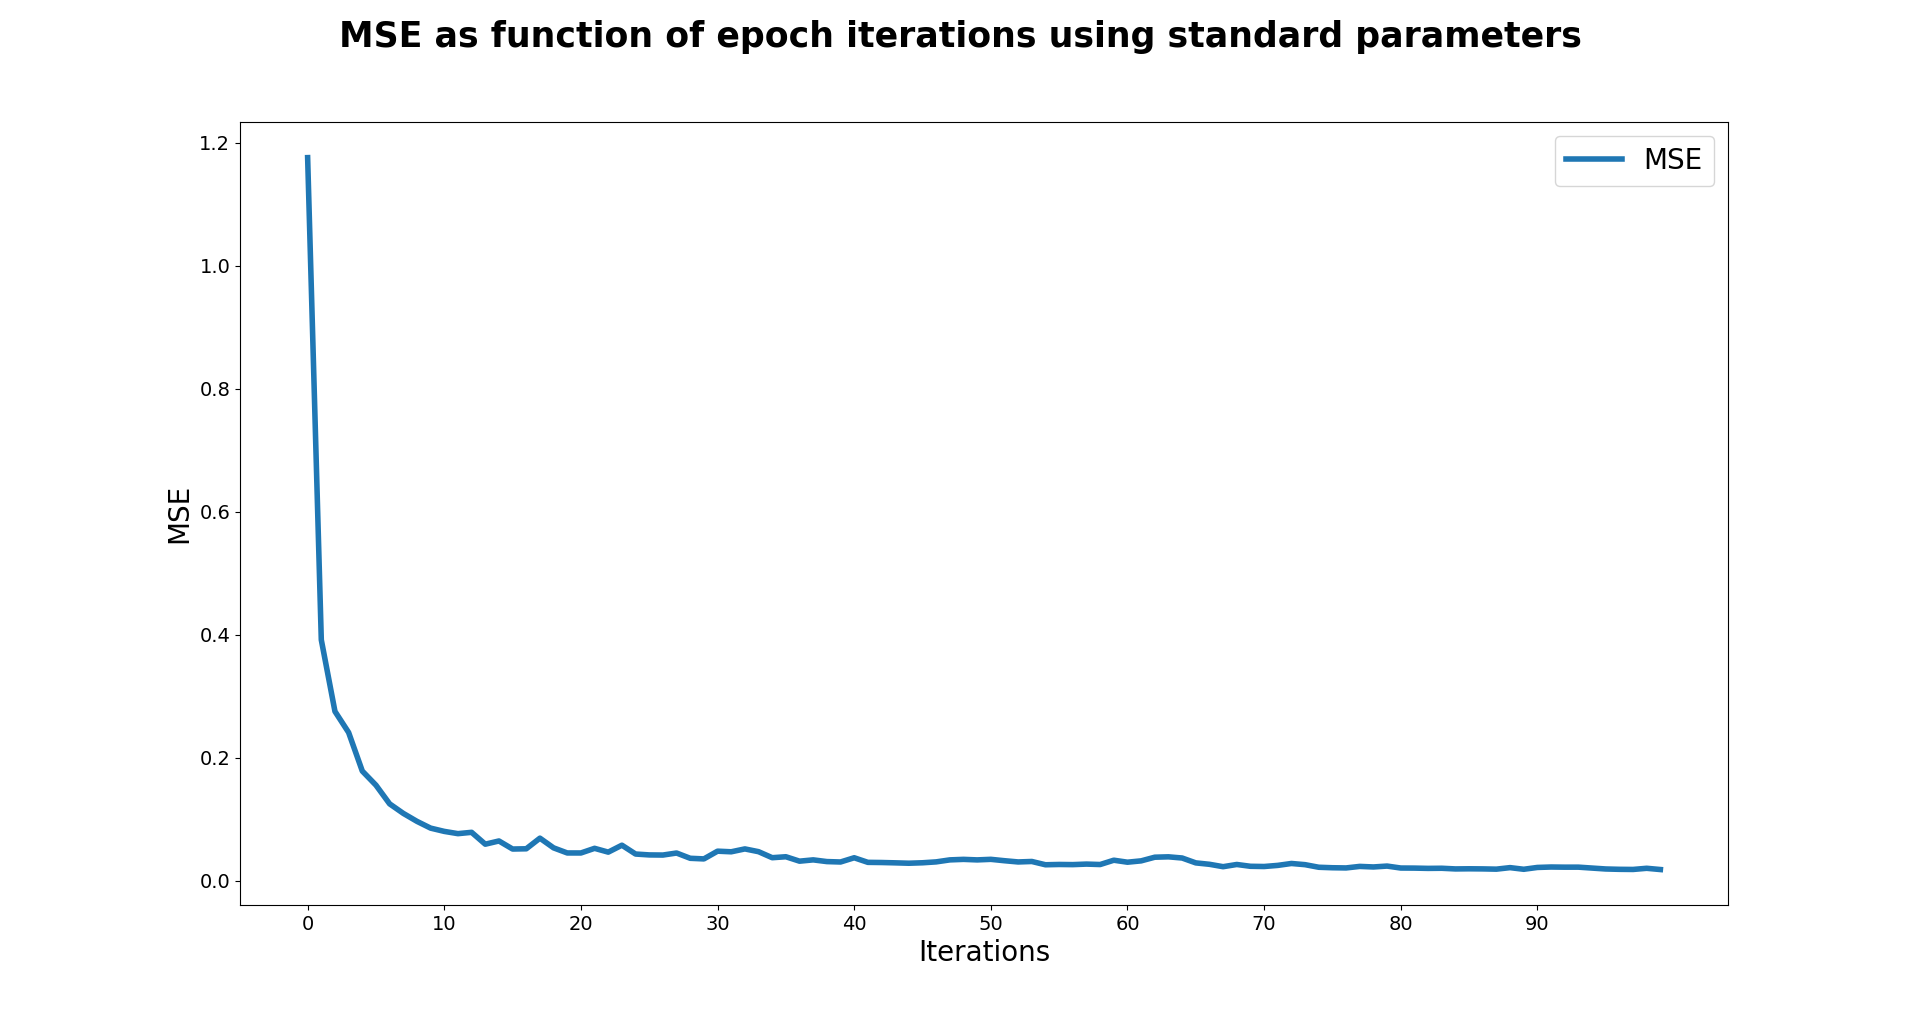
\includegraphics[width = 1\linewidth]{C:/Users/Sander/Documents/GitHub/FYS-STK4155/Project2/Project2/Report/Figures/MSEvsEPOCH_StandardRIDGE.PNG}
\caption{\label{fig:MSEvsEPOCHstandardRidge} The MSE as function of number of epoch iterations using static learning rate and Ridge equivalent SGD.}
\end{figure}

\noindent Figures \ref{fig:MSEvsEPOCHstandard} and \ref{fig:MSEvsEPOCHstandardRidge} shows that the MSE drastically increases as function of the number of epoch iterations, particularly at low number of iterations. At higher number of iterations, say around 30, the MSE keeps decreasing, but at a lower rate. One can also observe that the Ridge SGD starts at a lower MSE than the OLS SGD which indicate that Ridge algorithms fits the data better. Let us now see how the MSE changes as function of both epoch iterations and the size of the batch. We will then use the standard parameters, but change the batch size in the span $[100, 10, 1]$ and the results are shown in figures \ref{fig:MSEvsEPOCHbatchOLS} and \ref{fig:MSEvsEPOCHbatchRIDGE}

\begin{figure}[H]
\centering
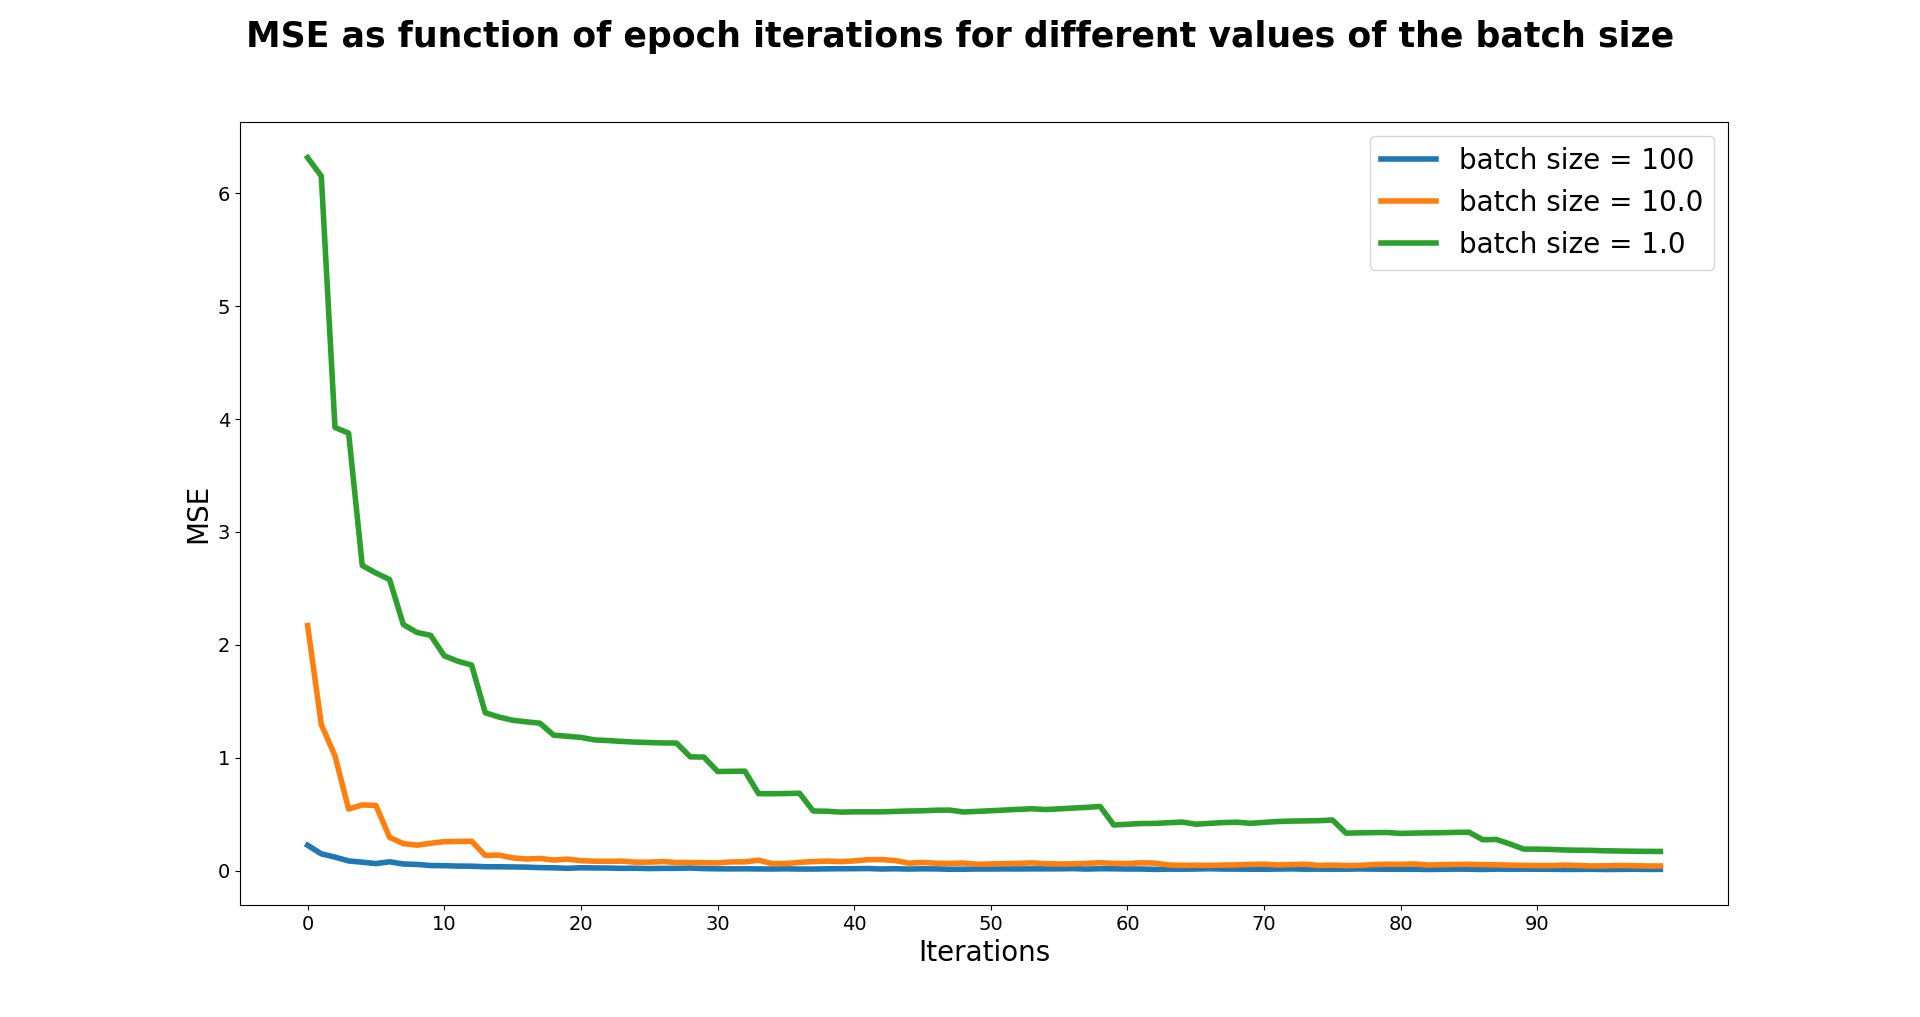
\includegraphics[width = 1\linewidth]{C:/Users/Sander/Documents/GitHub/FYS-STK4155/Project2/Project2/Report/Figures/MSEvsEPOCH_BatchOLS.PNG}
\caption{\label{fig:MSEvsEPOCHbatchOLS} The MSE as function of number of epoch iterations and batch sizes using static learning rate and OLS equivalent SGD.}
\end{figure}

\begin{figure}[H]
\centering
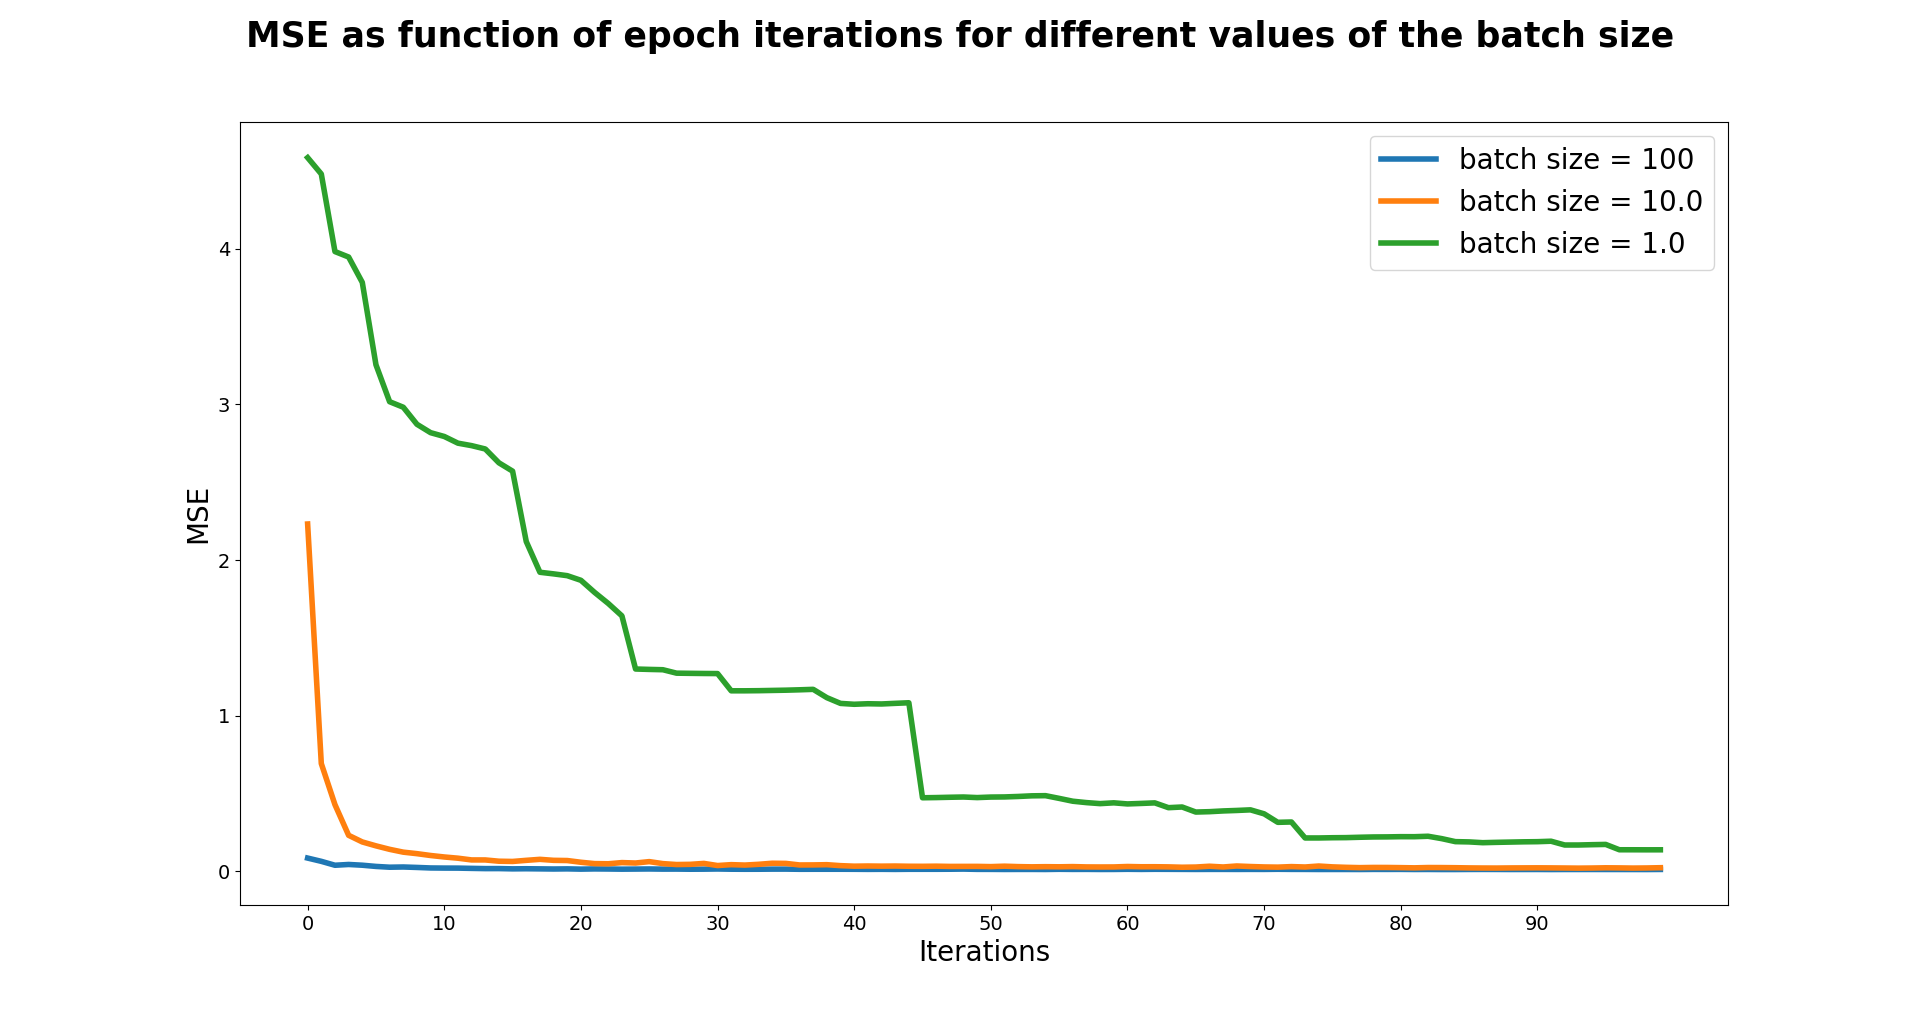
\includegraphics[width = 1\linewidth]{C:/Users/Sander/Documents/GitHub/FYS-STK4155/Project2/Project2/Report/Figures/MSEvsEPOCH_BatchRIDGE.PNG}
\caption{\label{fig:MSEvsEPOCHbatchRIDGE} The MSE as function of number of epoch iterations and batch sizes using static learning rate and Ridge equivalent SGD.}
\end{figure}

\noindent It can be observed from figures \ref{fig:MSEvsEPOCHbatchOLS} and \ref{fig:MSEvsEPOCHbatchRIDGE} that increasing the batch size drastically decreases the MSE. The batch size of 100 is equivalent to gradient descent (we use all observations) and it clearly has the lowest MSE for both the OLS and Ridge SGD. However, using the entirety of the data set can be extremely costly in terms of computational power, so it is not optimal for large data sets. What we also observe is that the difference in MSE between the batch sizes decreases for higher number of epoch iterations. In other words, we can utilize smaller batch sizes as long as we have a sufficiently large epoch. 
\\
Now let us see how the MSE varies as function of learning rate. We can again plot the MSE versus epoch iterations with our standard parameters, but vary the learning rate in the span $[0.0001, 0.001, 0.01]$

\begin{figure}[H]
\centering
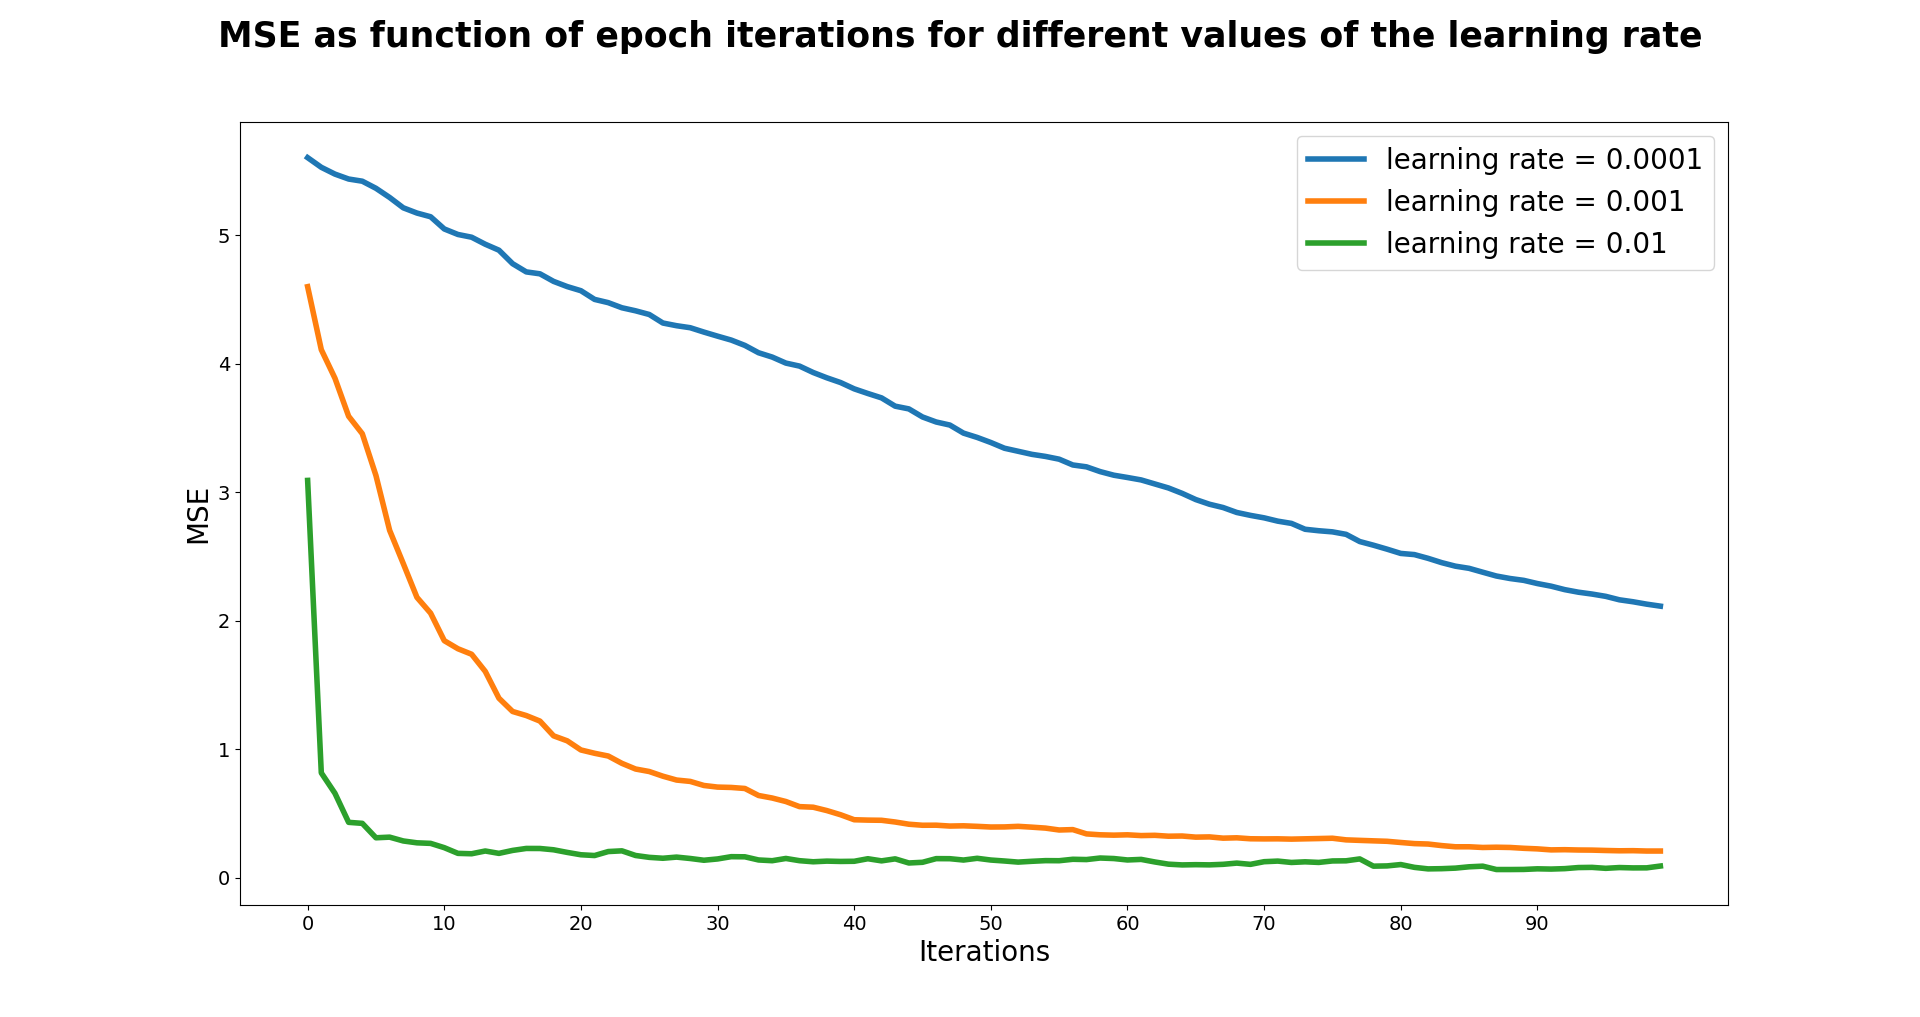
\includegraphics[width = 1\linewidth]{C:/Users/Sander/Documents/GitHub/FYS-STK4155/Project2/Project2/Report/Figures/MSEvsEPOCH_LearnOLS.PNG}
\caption{\label{fig:MSEvsEPOCHlaernOLS} The MSE as function of number of epoch iterations and learning rates using static learning rate and OLS equivalent SGD.}
\end{figure}

\begin{figure}[H]
\centering
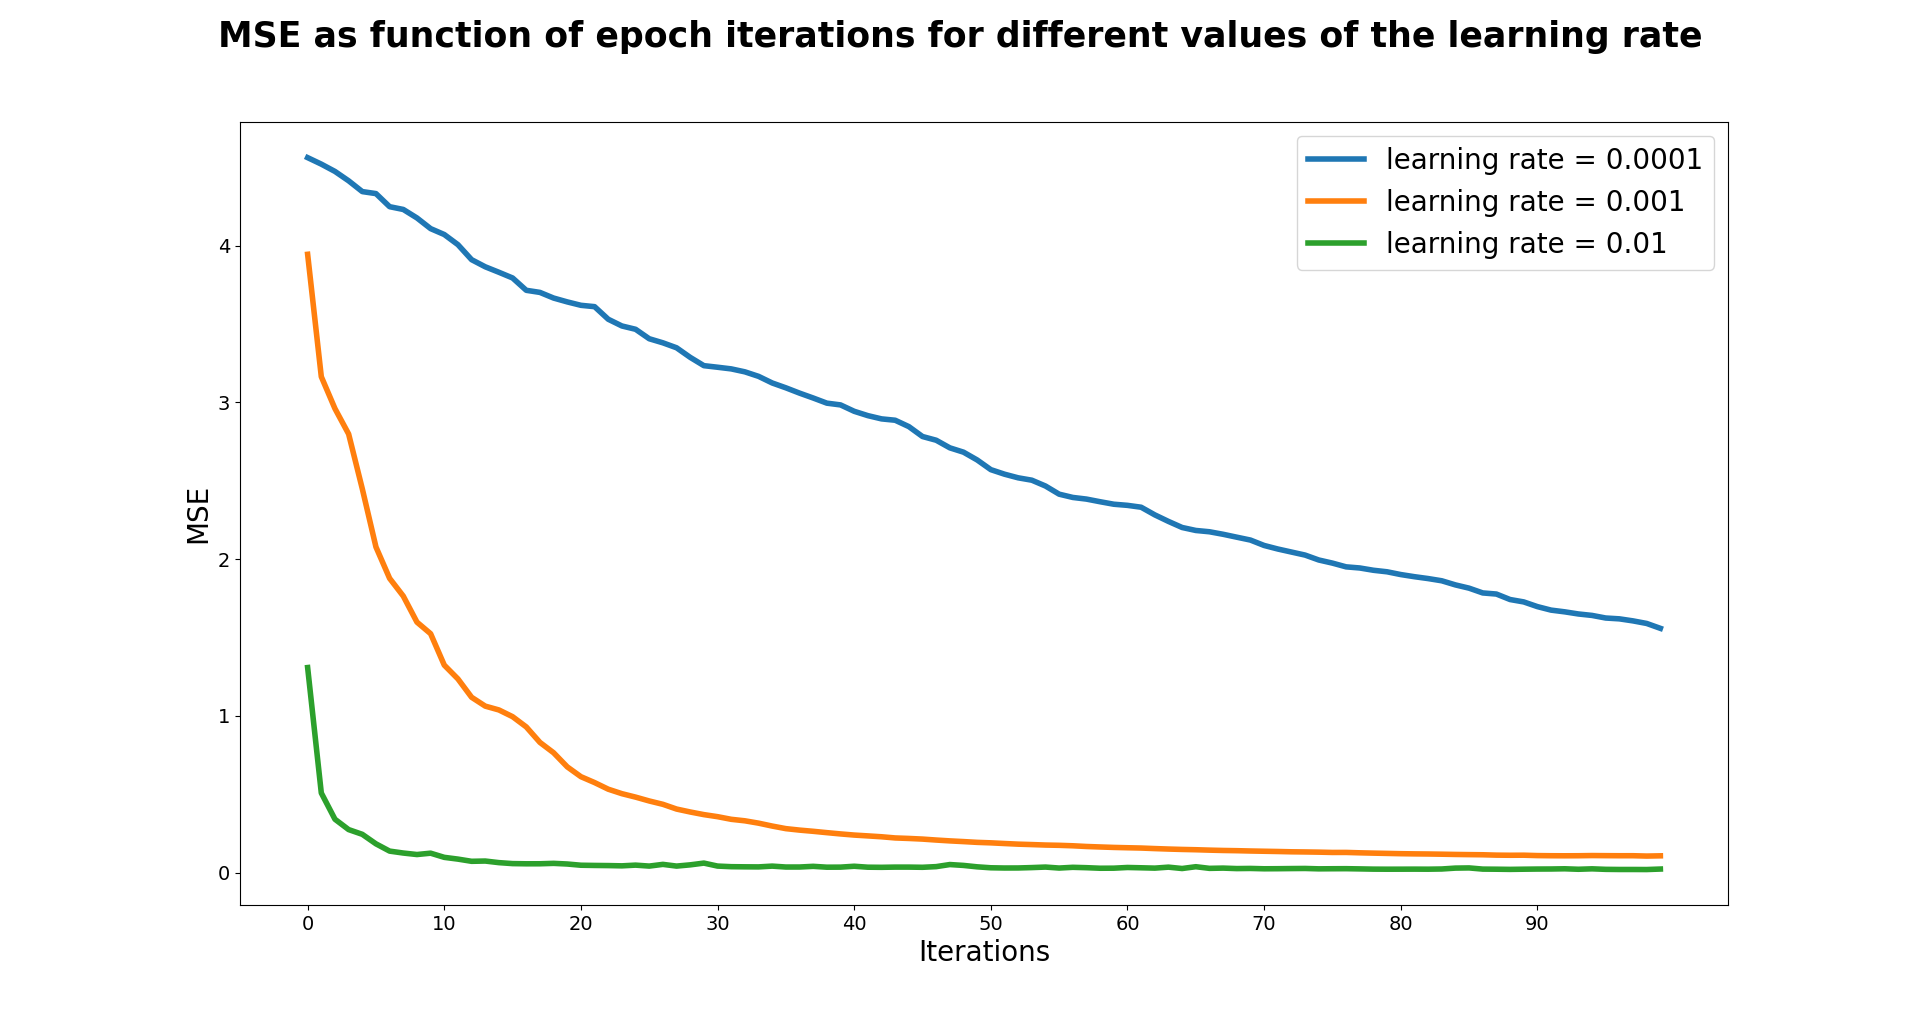
\includegraphics[width = 1\linewidth]{C:/Users/Sander/Documents/GitHub/FYS-STK4155/Project2/Project2/Report/Figures/MSEvsEPOCH_LearnRIDGE.PNG}
\caption{\label{fig:MSEvsEPOCHlearnRIDGE} The MSE as function of number of epoch iterations and learning rates using static learning rate and Ridge equivalent SGD.}
\end{figure}

\noindent One can observe from figures \ref{fig:MSEvsEPOCHlaernOLS} and \ref{fig:MSEvsEPOCHlearnRIDGE} that increasing the learning rate decreases the MSE for a low number of epoch iterations. However, the MSE of learning rates $0.01$ and $0.001$ converge for a higher number of epoch iterations. The MSE of the learning rate $0.0001$ does not drop exponentially, but linearly. This may be due to the learning rate is so small that the SGD takes a very long time to reach any kind of minimum, making the process too slow for the number of epoch iterations shown here. What we observe overall is that a learning rate anywhere over $0.001$ is fine as long as we have sufficiently many epoch iterations. 
\\
We can also study the how the MSE of the Ridge SGD changes as function of the number of epoch iterations and the penalty parameter $\lambda$. We again use the standard parameters but change the penalty parameter in the span $[0.0001, 0.001, 0.01, 0.1, 1]$ and the results are shown in figure \ref{fig:MSEvsEPOCHlambRIDGE}

\begin{figure}[H]
\centering
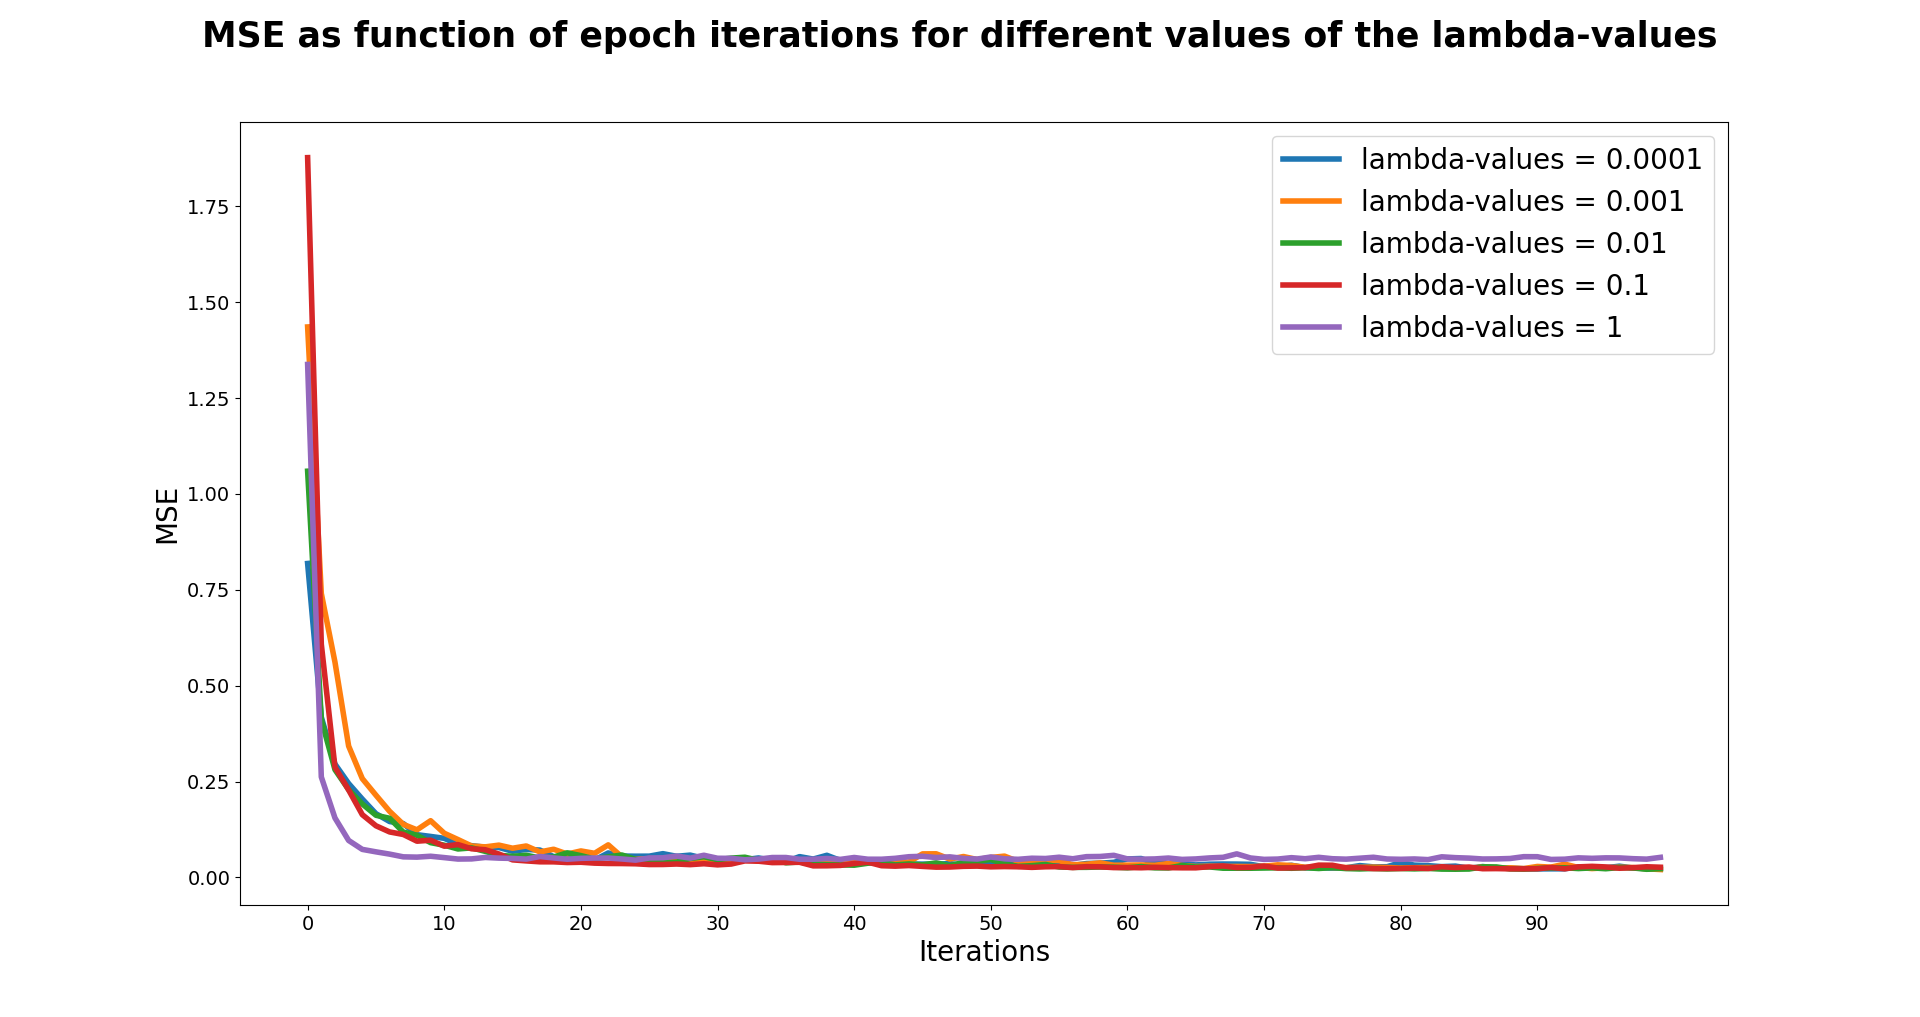
\includegraphics[width = 1\linewidth]{C:/Users/Sander/Documents/GitHub/FYS-STK4155/Project2/Project2/Report/Figures/MSEvsEPOCH_lambRIDGE.PNG}
\caption{\label{fig:MSEvsEPOCHlambRIDGE} The MSE as function of number of epoch iterations and penalty parameter $\lambda$ using static learning rate and Ridge equivalent SGD.}
\end{figure}

\noindent One can observe from figure \ref{fig:MSEvsEPOCHlambRIDGE} that the different penalty parameters yields similar results. One interesting observations is that the penalty parameter of $1$ yields the lowest MSE for a low number of epoch iterations, while it yields the highest MSE for a high number of epoch iterations. This may be caused by the fact that some of the regression coefficients are set close to zero and therefore do not contribute much to the overall cost function. It may be that the minimum of this reduced cost function has a minimum or local minimum with higher MSE than that of the less reduced cost function.

\begin{center}
\large{\textbf{Parameter dependencies for scheduled learning rate}}
\end{center}

\noindent We now aim to repeat the above analysis, but with a scheduled/adaptive learning rate. The learning rate will change as according to $\frac{t_0}{t+t_1}$ where $t_0 = 5$, $t_1 = 50$ and where t is constantly changing as function of epoch and batch iterations such that $t = $ current epoch iteration $\times$ batch size $+$ current batch iteration. The hopes for the scheduled learning rate is that we take large steps when we are far from the minimum of the cost function, while we take smaller steps as we approach said minimum. This will decrease our chances of getting "stuck" in some local minimum as our steps are too large for us to find ourselves in such a local minimum. We can implement this schedule in the SGD algorithm and see how the MSE changes for different epoch iterations and varying parameters. We start by simply plotting the MSE as function of epoch iteration using the standard parameters of table \ref{tab:standardParam}

\begin{figure}[H]
\centering
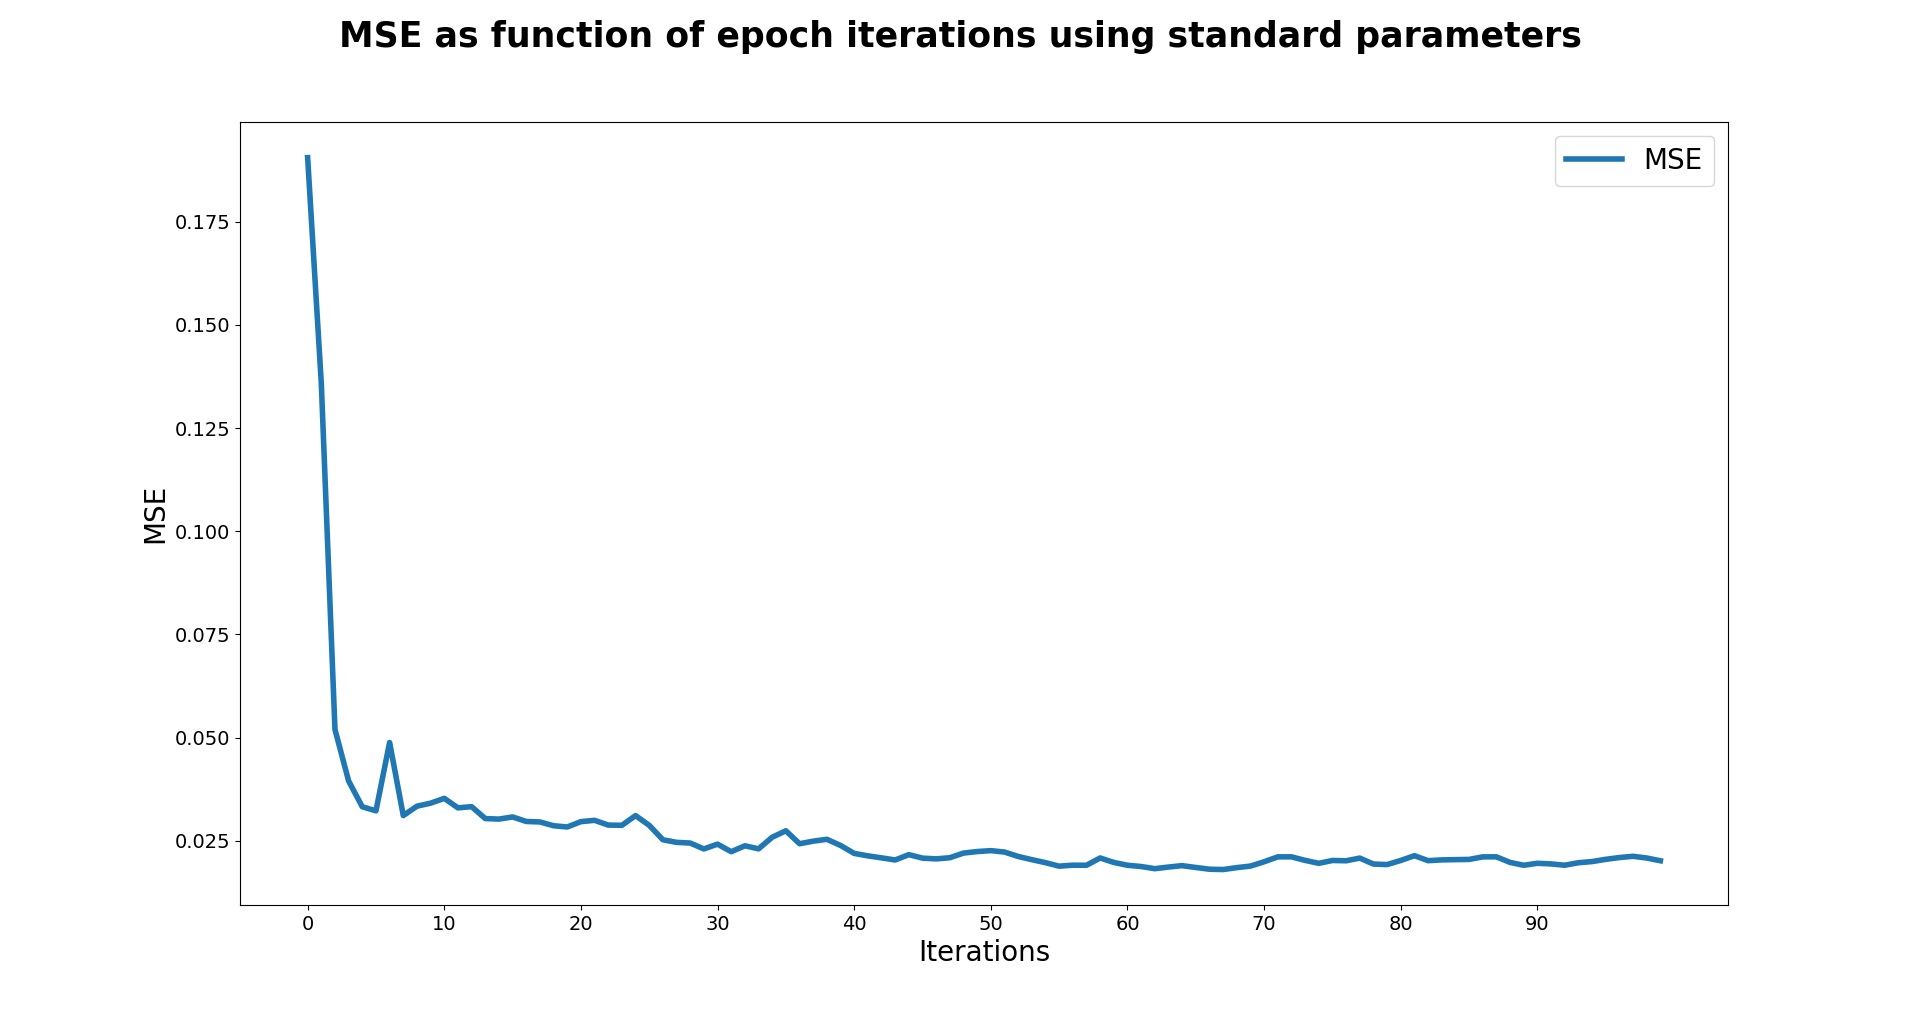
\includegraphics[width = 1\linewidth]{C:/Users/Sander/Documents/GitHub/FYS-STK4155/Project2/Project2/Report/Figures/MSEvsEPOCH_StandardOLS_schedule.PNG}
\caption{\label{fig:MSEvsEPOCHstandard_sch} The MSE as function of number of epoch iterations using a learning schedule rate and OLS equivalent SGD.}
\end{figure}

\begin{figure}[H]
\centering
\includegraphics[width = 1\linewidth]{C:/Users/Sander/Documents/GitHub/FYS-STK4155/Project2/Project2/Report/Figures/MSEvsEPOCH_StandardRIDGE_schedule.PNG}
\caption{\label{fig:MSEvsEPOCHstandardRidge_sch} The MSE as function of number of epoch iterations using a learning schedule rate and Ridge equivalent SGD.}
\end{figure}

\noindent It can be observed when comparing figures \ref{fig:MSEvsEPOCHstandard} and \ref{fig:MSEvsEPOCHstandardRidge} to figures \ref{fig:MSEvsEPOCHstandard_sch} and \ref{fig:MSEvsEPOCHstandardRidge_sch} that the MSE drops much quicker when we utilize a learning schedule. This is a direct consequence of taking larger steps when we are far away from the minimum. This ultimately leads to fewer steps to get to the minimum of the cost function. 
\\
We can also study how the MSE changes as function of batch size when we utilize a learning schedule and the result is plotted in figures QQQ and QQQ

\begin{figure}[H]
\centering
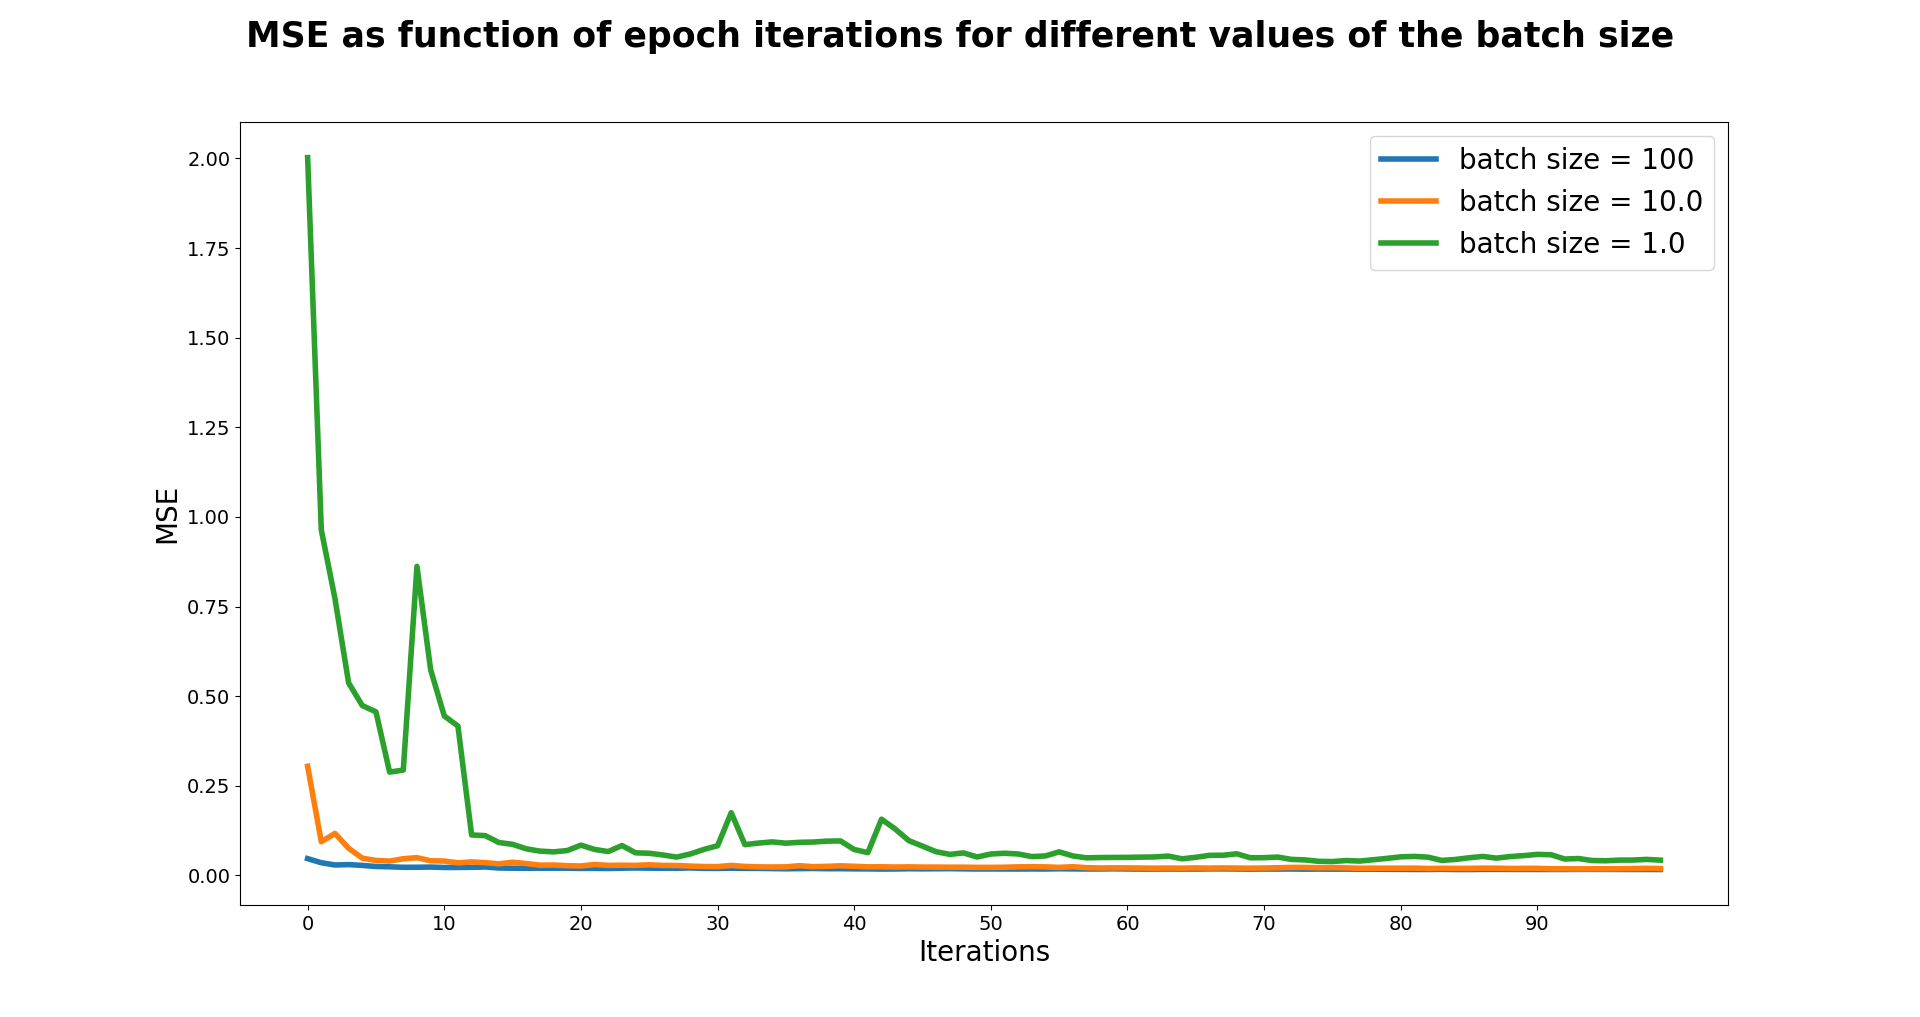
\includegraphics[width = 1\linewidth]{C:/Users/Sander/Documents/GitHub/FYS-STK4155/Project2/Project2/Report/Figures/MSEvsEPOCH_BatchOLS_schedule.PNG}
\caption{\label{fig:MSEvsEPOCHbatchOLS_sch} The MSE as function of number of epoch iterations and batch sizes using a learning schedule and OLS equivalent SGD.}
\end{figure}

\begin{figure}[H]
\centering
\includegraphics[width = 1\linewidth]{C:/Users/Sander/Documents/GitHub/FYS-STK4155/Project2/Project2/Report/Figures/MSEvsEPOCH_BatchRIDGE_schedule.PNG}
\caption{\label{fig:MSEvsEPOCHbatchRIDGE_sch} The MSE as function of number of epoch iterations and batch sizes using a learning schedule and Ridge equivalent SGD.}
\end{figure}

\noindent When we compare figures \ref{fig:MSEvsEPOCHbatchOLS} and \ref{fig:MSEvsEPOCHbatchRIDGE} to figures \ref{fig:MSEvsEPOCHbatchOLS_sch} and \ref{fig:MSEvsEPOCHbatchRIDGE_sch} we can observe that the batch size seems to play a more important role when using a learning schedule as the gap between batchs sizes are much greater than that of static learning rate. What is also observed is that the a batch size of one observation is much more "jagged" when we utilize a learning schedule. This be caused by the schedule "jumping" in and out of local minimums of the cost function. We can look at batch size equal to one for the OLS SGD in figure \ref{fig:MSEvsEPOCHbatchOLS_sch} where the MSE initially decreases a lot to around 5 iterations, but then has a large upturn in MSE. This may be one of these local minimum the algorithm found itself in. However, it does seem that the algorithm eventually finds the absolute minimum of the entire cost function as the "jagged" parts disappear for higher epoch iterations. 
\\
This phenomena seems to be a greater problem for the OLS as the Ridge SGD is nowhere near as jagged as the OLS SGD for batch size equal to one. This may be caused by the fact that some variables are reduced to a very small value, thereby removing any local minimum in that particular dimension.
\\
We can investigate the ridge implementation further by plotting plotting the MSE versus the epoch iterations for different values of the penalty parameter $\lambda$

\begin{figure}[H]
\centering
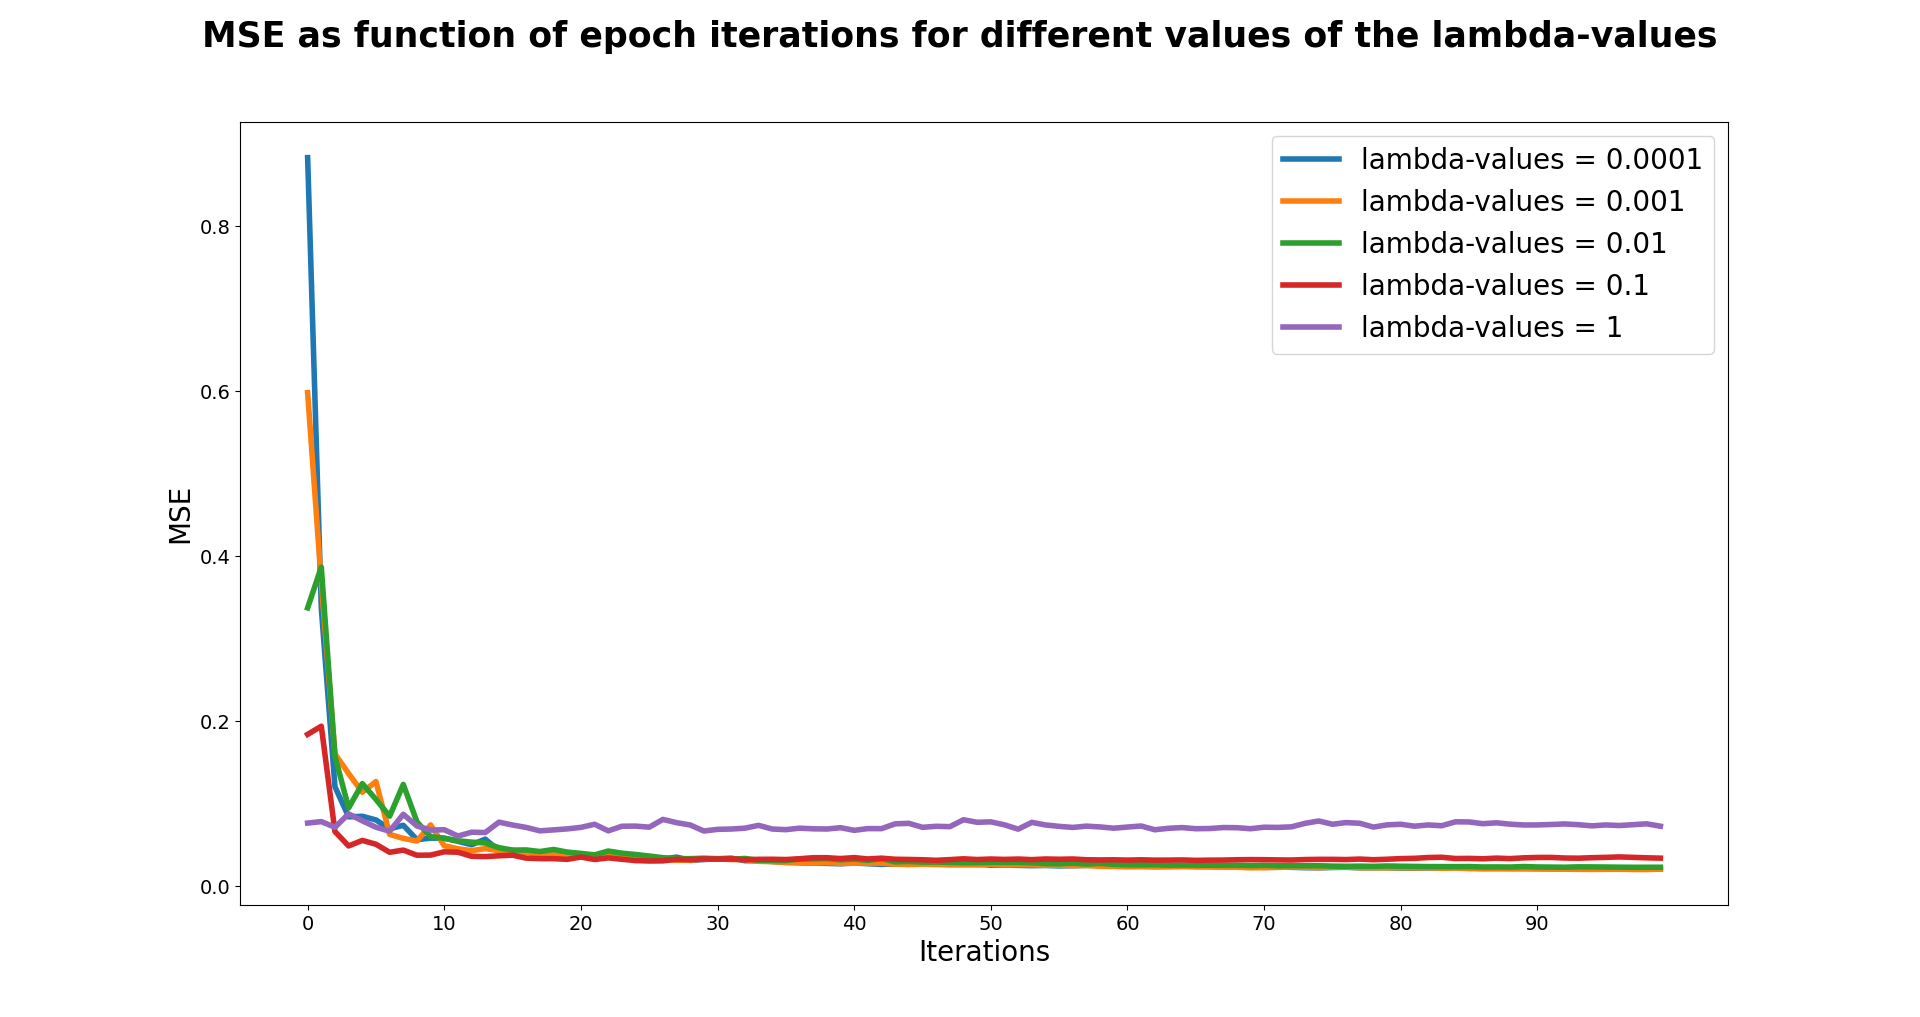
\includegraphics[width = 1\linewidth]{C:/Users/Sander/Documents/GitHub/FYS-STK4155/Project2/Project2/Report/Figures/MSEvsEPOCH_lambRIDGE_schedule.PNG}
\caption{\label{fig:MSEvsEPOCHlambRIDGE_sch} The MSE as function of number of epoch iterations and penalty parameter $\lambda$ using a learning schedule and Ridge equivalent SGD.}
\end{figure}

\begin{figure}[H]
\centering
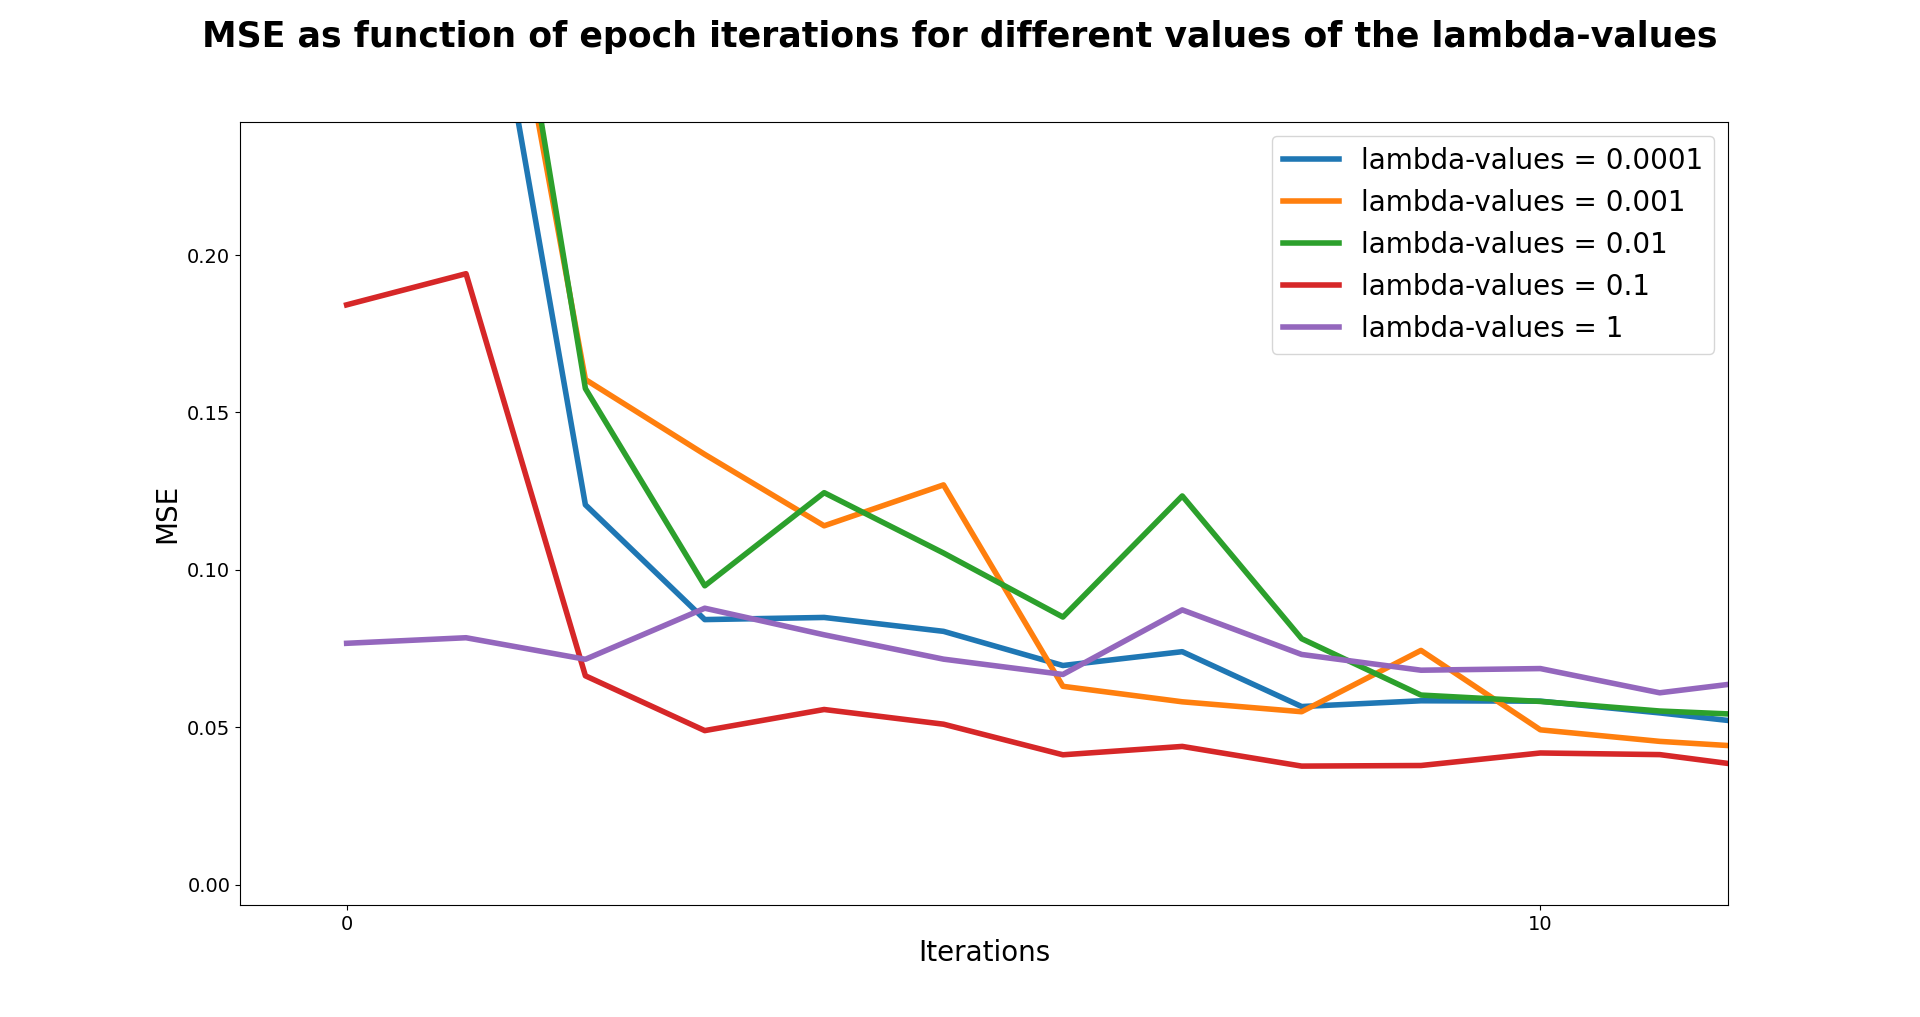
\includegraphics[width = 1\linewidth]{C:/Users/Sander/Documents/GitHub/FYS-STK4155/Project2/Project2/Report/Figures/MSEvsEPOCH_lambRIDGE_schedule2.PNG}
\caption{\label{fig:MSEvsEPOCHlambRIDGE_sch2} The MSE as function of number of epoch iterations and penalty parameter $\lambda$ using a learning schedule and Ridge equivalent SGD. This is a zoom-in of figure \ref{fig:MSEvsEPOCHlambRIDGE_sch}}.
\end{figure}

\noindent We can observe from figures that the choice of penalty parameter $\lambda$ has little or no effect on the MSE, except for when $\lambda = 1$. The MSE in this case never really increase or decrease, which is probably caused by the penalty term setting too many regression coefficients close to zero, meaning there is not really a minimum of the cost function since if all the regression coefficients are to small. 
\\
We also observe that the MSE for penalty parameters less than one decrease their MSE at a very low number of epoch iterations. Indicating that the minimum value is easy to find when some variables are very small.

\newpage

\begin{center}
\Large{\textbf{Exercise 1b): Neural network for regression}}
\end{center}

\begin{center}
\large{\textbf{The basics of a neural network}}
\end{center}

\noindent A neural network is a concept based on how neurons operate in the brain where we have an input that travels through neurons that weights the input, eventually making its way to some given set of neuron that trigger an output. This process can be replicated by computers by creating a layered model consisting of one input layer where the data goes in, an output layer where the neural network prediction comes out and a given number of hidden layers consisting of hidden neurons. A conceptual drawing of this process can be seen in figure \ref{fig:nnconcept}

\begin{figure}[H]
\centering
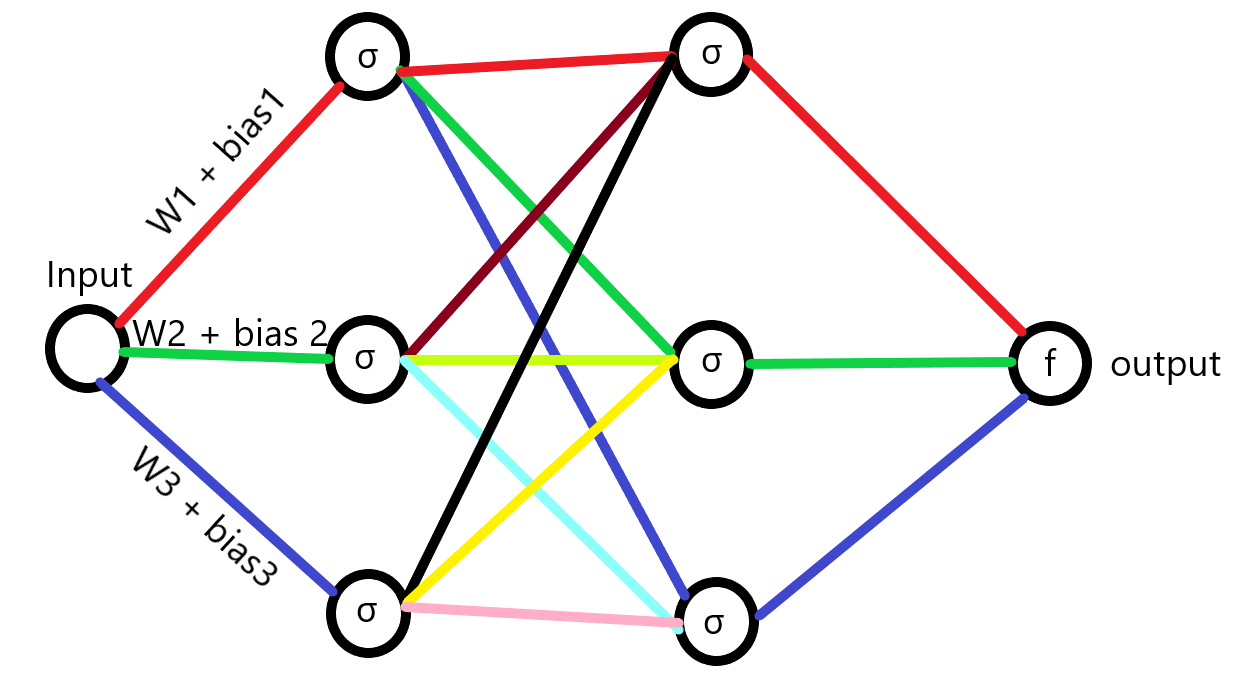
\includegraphics[width = 1\linewidth]{C:/Users/Sander/Documents/GitHub/FYS-STK4155/Project2/Project2/Report/Figures/NeuralNetConcept.PNG}
\caption{\label{fig:nnconcept} Conseptual drawing of a neural network. Here we have one input layer, two hidden layers and one output layer. The input and output layers consist of a single neuron, while the hidden layers have three neurons each. The input to each neuron is a weighted sum (W) plus a bias (B) from the previous layer. The output of a given neuron is the input to that neuron going through a activation function $\sigma$ which is then passed to the neurons in the next layer. The output activation function may be different than that of the neuron activation functions.}
\end{figure}

\noindent Figure \ref{fig:nnconcept} shows an input layer that passes a weighted sum plus bias to the three neurons in the first hidden layer. The weights $W_1, W_2$ and $W_3$ are typically different while the biases $B_1, B_2$ and $B_3$ are typically the equal. When these weighted sums plus bias enter a neuron, they are passed through an activation function which compresses the input to some value between zero and one. It is intuitive to think of this as how activated a neuron is, where one being fully activated and zero being fully inactivated. The data is passed through every neuron in every layer and will eventually reach the output layer where another activation function is applied. This whole process is called feed forward and is typically the first step of any neural network algorithm.
\\
The next step is to tune the weights within the neural network. This is where the gradient descent from exercise 1a) comes in. We can utilize the stochastic gradient descent to find the minimum of a cost function where each dimension is the weights of the neural network. Can then find which value of the weight would incrementally decrease the cost function, and then go back though our neural network and update the weight values in each neuron. This process is often called back propagation. We want to repeat the feed forward and back propagation many times in order for the weight to find their optimal value. This is called the training of the neural network. When we have trained the neural network sufficiently, it can be used to predict new data the network has never seen before. With these processes in mind, we can implement an algorithm that performs feed forward and back propagation.

\begin{center}
\large{\textbf{Set-up of our neural network}}
\end{center}

\noindent We now aim to implement a neural network code, but first we must decide what the parameters of the network should be. The initial values of the weights are simply drawn randomly from a normal distribution and each neuron has its own weight. The bias has in this case simply been set to $0.01$. The role of the bias is to make sure there is some input to the neurons. Say a neuron only receives zeros from the previous layer. This would in turn lead to a feed forward of only zeros for that particular set of neurons meaning they will never contribute to the network. Therefore, it is important to add some bias to each neuron. 
\\
The activation function in the hidden layer will be the sigmoid function which is given by equation \ref{eq:sig}

\begin{equation}\label{eq:sig}
\begin{aligned}
\frac{1}{1 + e^{-x}}
\end{aligned}
\end{equation}

\noindent It can be seen from the definition of the sigmoid function that whatever the value of x, the output is always somewhere between zero and one. We can utilize this to force the neurons to output a value between zero and one.
\\
The activation function for the output layer is simply a linear function that return itself, i.e. there is no activation function. This is because we essentially performing linear regression, and the output function must therefore be the same shape as the input.
\\
The input will in this case be the Franke function of dimensions $100 \times 100$ and so the output must also be of dimensions $100 \times 100$. 

\begin{center}
\large{\textbf{Neural network results}}
\end{center}

\noindent After implementing the neural network described in the previous section, we can analyse the results by plotting the MSE and $R^2$ for different learning rates for the SGD regression scheme, the neural network implementation and the Scikit neural network implementation for both the OLS and Ridge case as seen in figures \ref{fig:MSEvsLearn_OLS}, \ref{fig:MSEvsLearn_Ridge}, \ref{fig:R2vsLearn_OLS} and \ref{fig:R2vsLearn_Ridge} 

\begin{figure}[H]
\centering
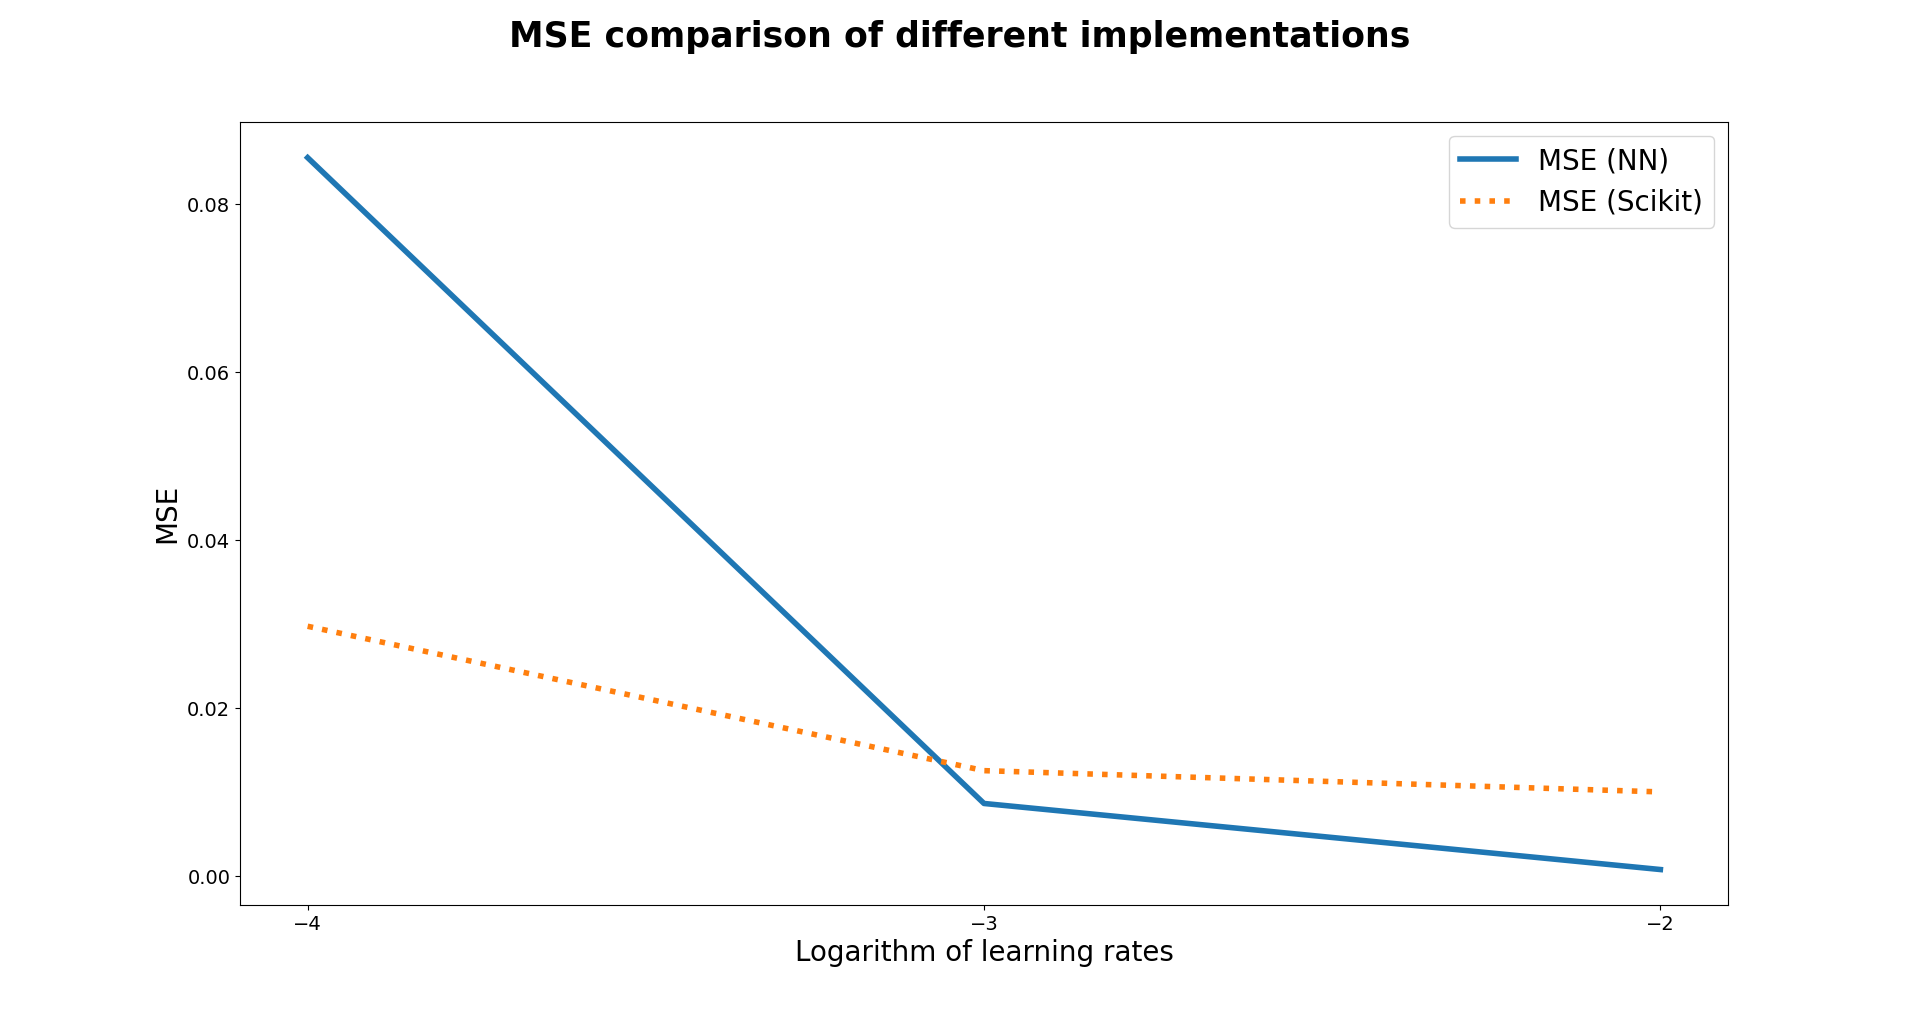
\includegraphics[width = 1\linewidth]{C:/Users/Sander/Documents/GitHub/FYS-STK4155/Project2/Project2/Report/Figures/MSEvsLearn_OLS.PNG}
\caption{\label{fig:MSEvsLearn_OLS} The MSE as function of different learning rates for the SGD regression scheme, the neural network implementation and the Scikit neural network implementation. Here we have utilized the OLS implementation.}
\end{figure}

\begin{figure}[H]
\centering
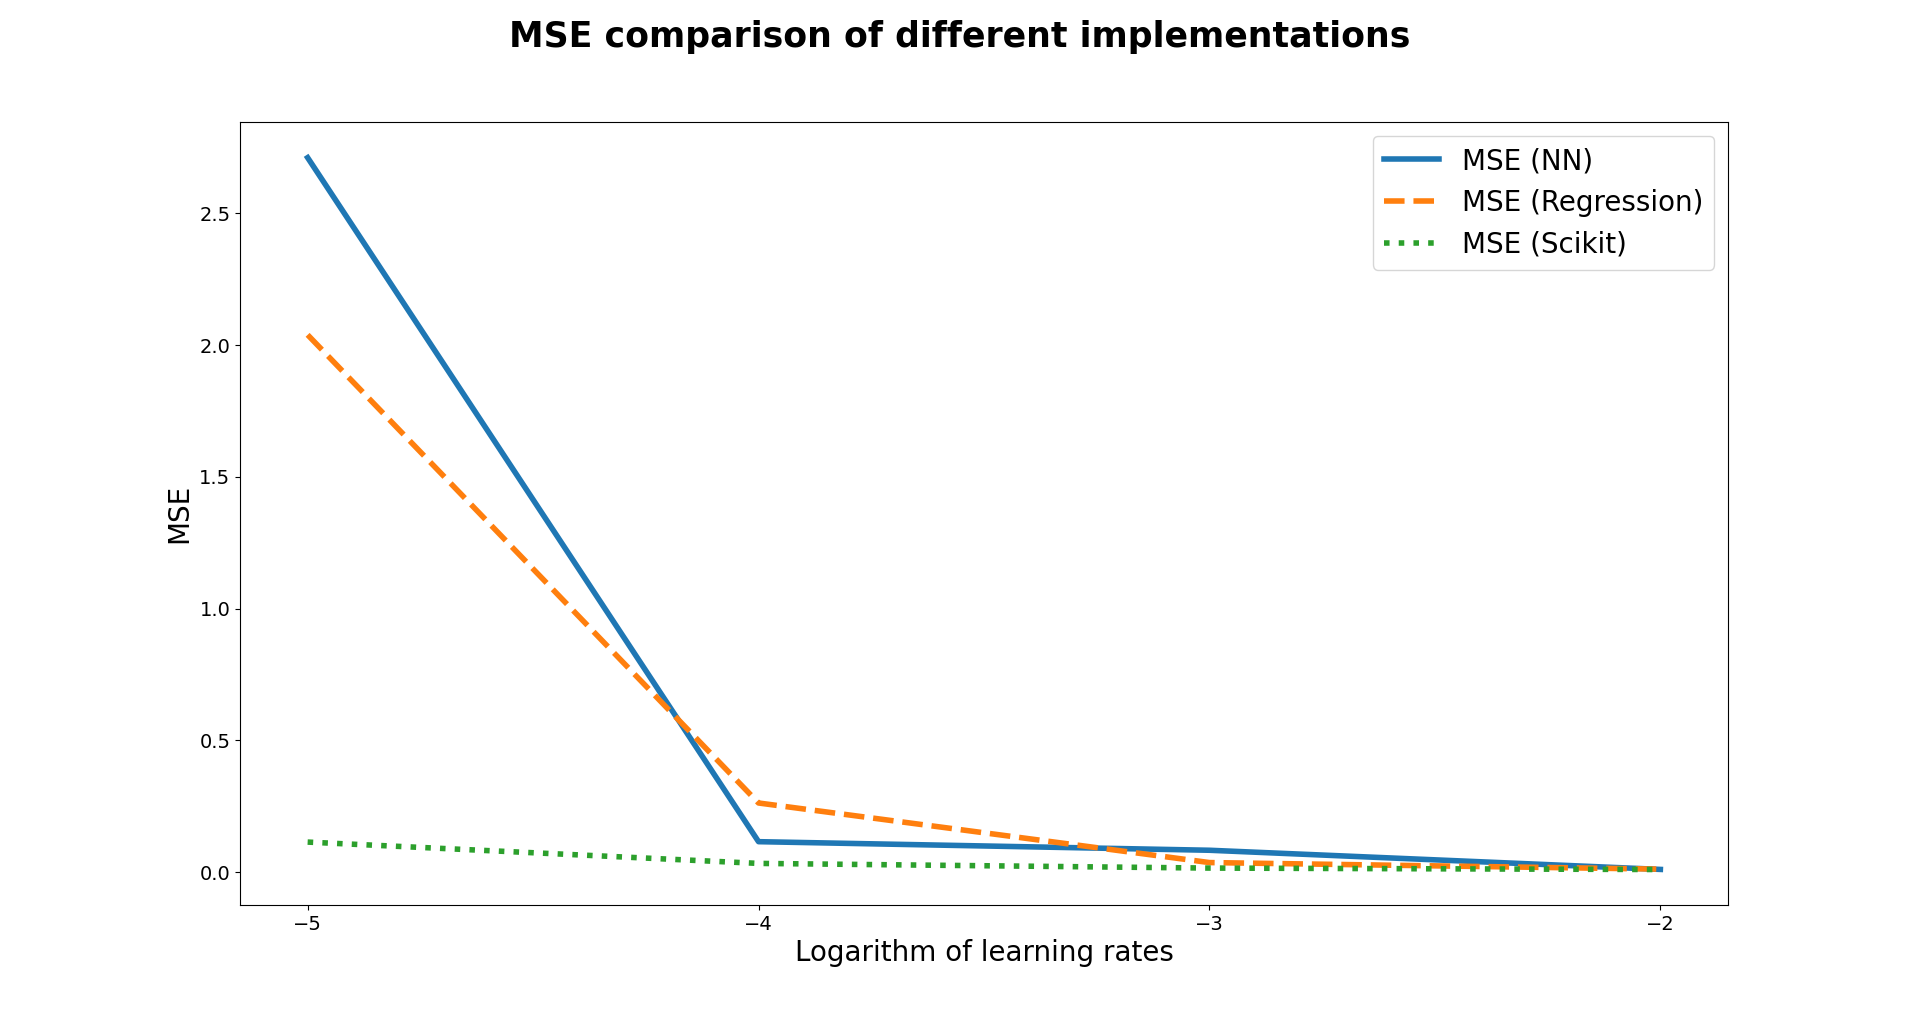
\includegraphics[width = 1\linewidth]{C:/Users/Sander/Documents/GitHub/FYS-STK4155/Project2/Project2/Report/Figures/MSEvsLearn_Ridge.PNG}
\caption{\label{fig:MSEvsLearn_Ridge} The MSE as function of different learning rates for the SGD regression scheme, the neural network implementation and the Scikit neural network implementation. Here we have utilized the Ridge implementation.}
\end{figure}

\begin{figure}[H]
\centering
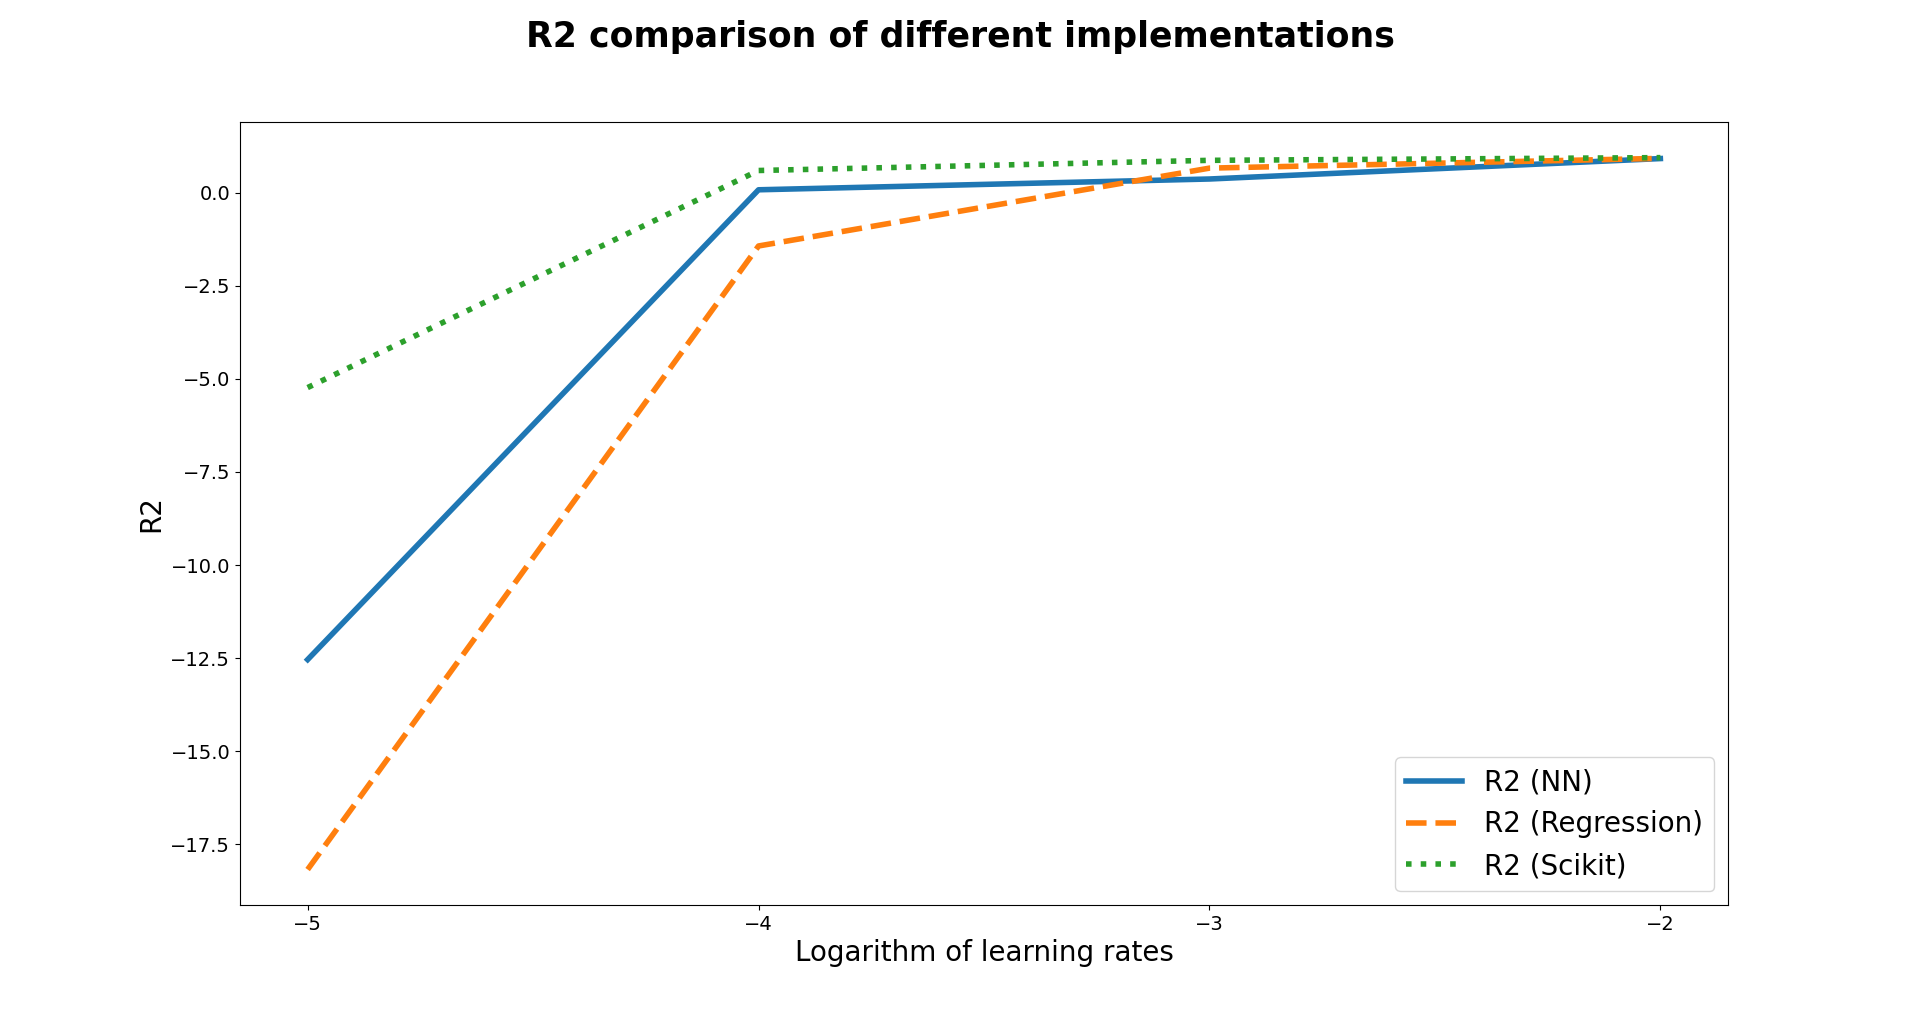
\includegraphics[width = 1\linewidth]{C:/Users/Sander/Documents/GitHub/FYS-STK4155/Project2/Project2/Report/Figures/R2vsLearn_OLS.PNG}
\caption{\label{fig:R2vsLearn_OLS} The $R^2$ as function of different learning rates for the SGD regression scheme, the neural network implementation and the Scikit neural network implementation. Here we have utilized the OLS implementation.}
\end{figure}

\begin{figure}[H]
\centering
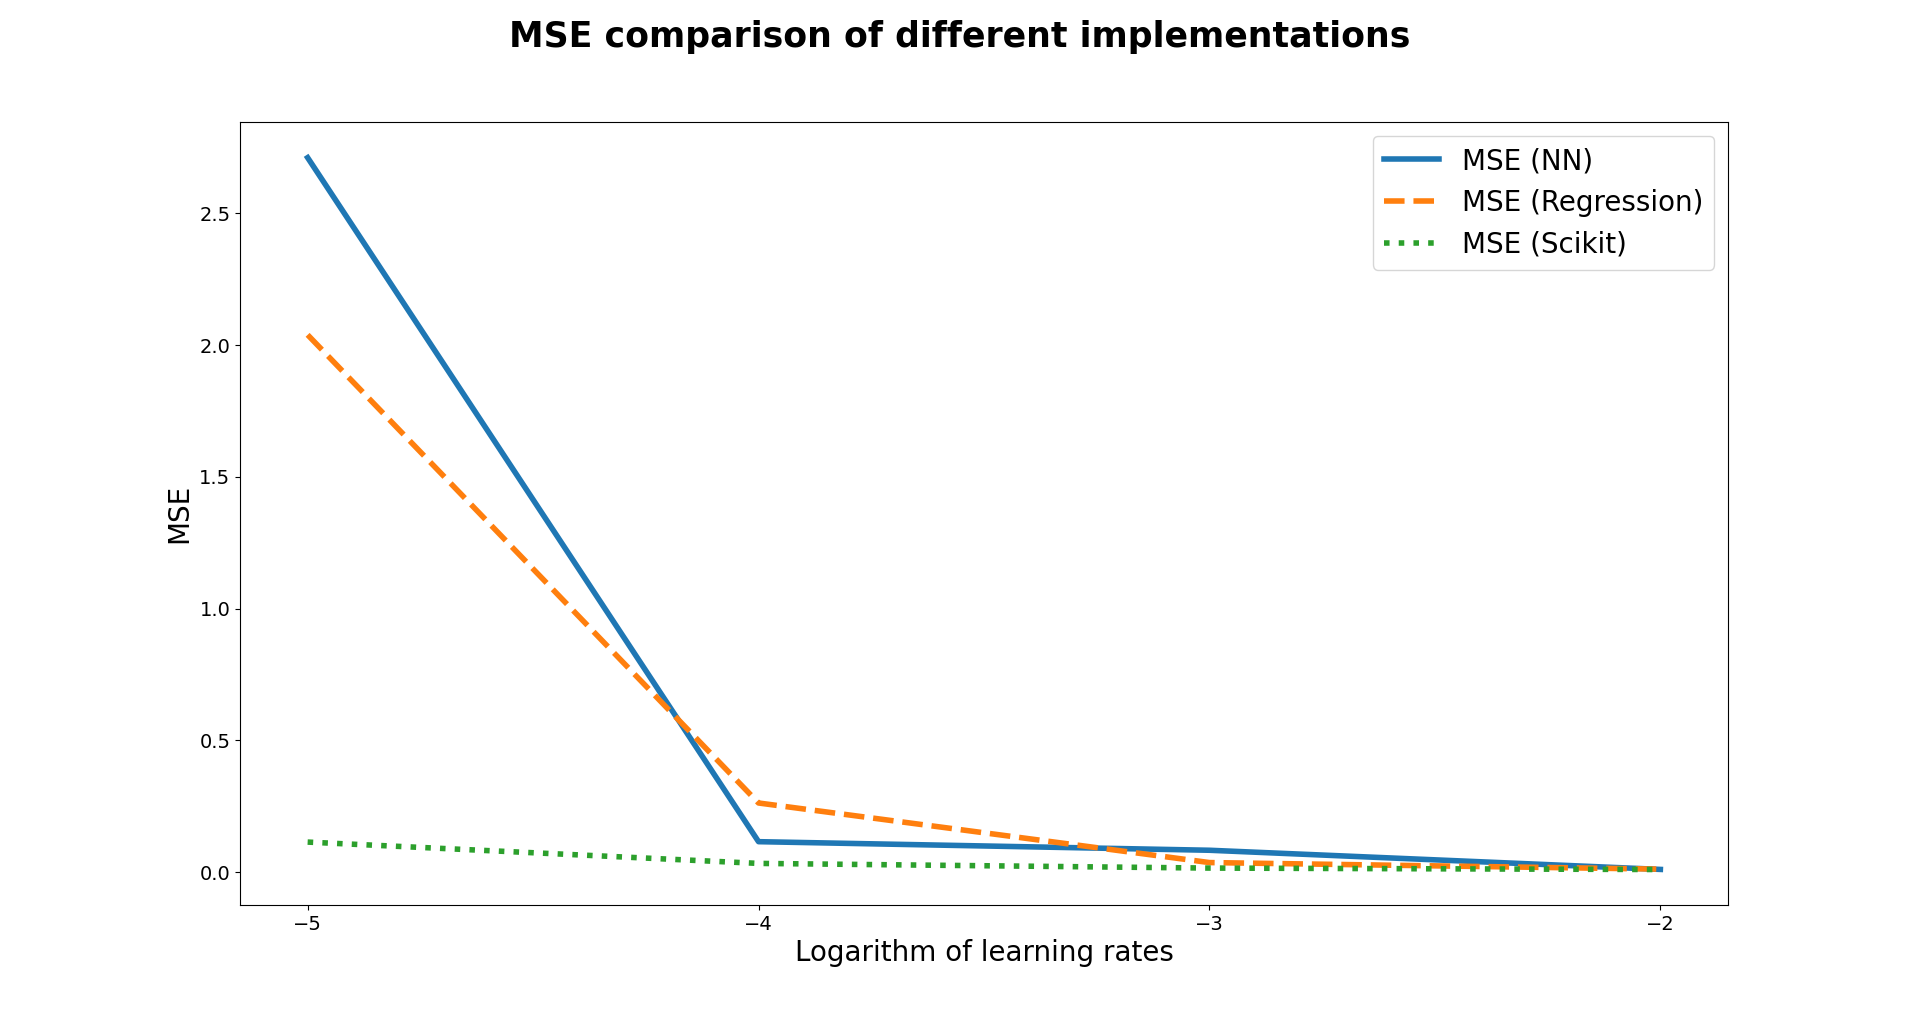
\includegraphics[width = 1\linewidth]{C:/Users/Sander/Documents/GitHub/FYS-STK4155/Project2/Project2/Report/Figures/MSEvsLearn_Ridge.PNG}
\caption{\label{fig:R2vsLearn_Ridge} The $R^2$ as function of different learning rates for the SGD regression scheme, the neural network implementation and the Scikit neural network implementation. Here we have utilized the Ridge implementation.}
\end{figure}

\noindent One can observe from figures \ref{fig:MSEvsLearn_OLS} and \ref{fig:MSEvsLearn_Ridge} that the MSE for all three methods are about equal for learning rates over $0.001$. However, when we decrease the learning rate below this value, we see a sharp contrast. Here, the Scikit neural network implementation performs the best for both Ridge and OLS. The regression and my own neural network seems to perform about the same for Ridge regression, but my neural network outperforms the regression in the OLS case. This is confirmed by by the $R^2$ plots in figures \ref{fig:R2vsLearn_OLS} and \ref{fig:R2vsLearn_Ridge}. The optimal MSE and $R^2$ is found at learning rate equal to $0.01$ and this will be utilized in the following analysis.
\\
We now aim to find what number of hidden layers and hidden neurons give us the lowest MSE. The following figures shows MSE and $R^2$ heat maps for different number of hidden layers and hidden neurons using the optimal learning rate of $0.01$ using both OLS and Ridge for both my own and Scikit implementations.

\begin{figure}[H]
\centering
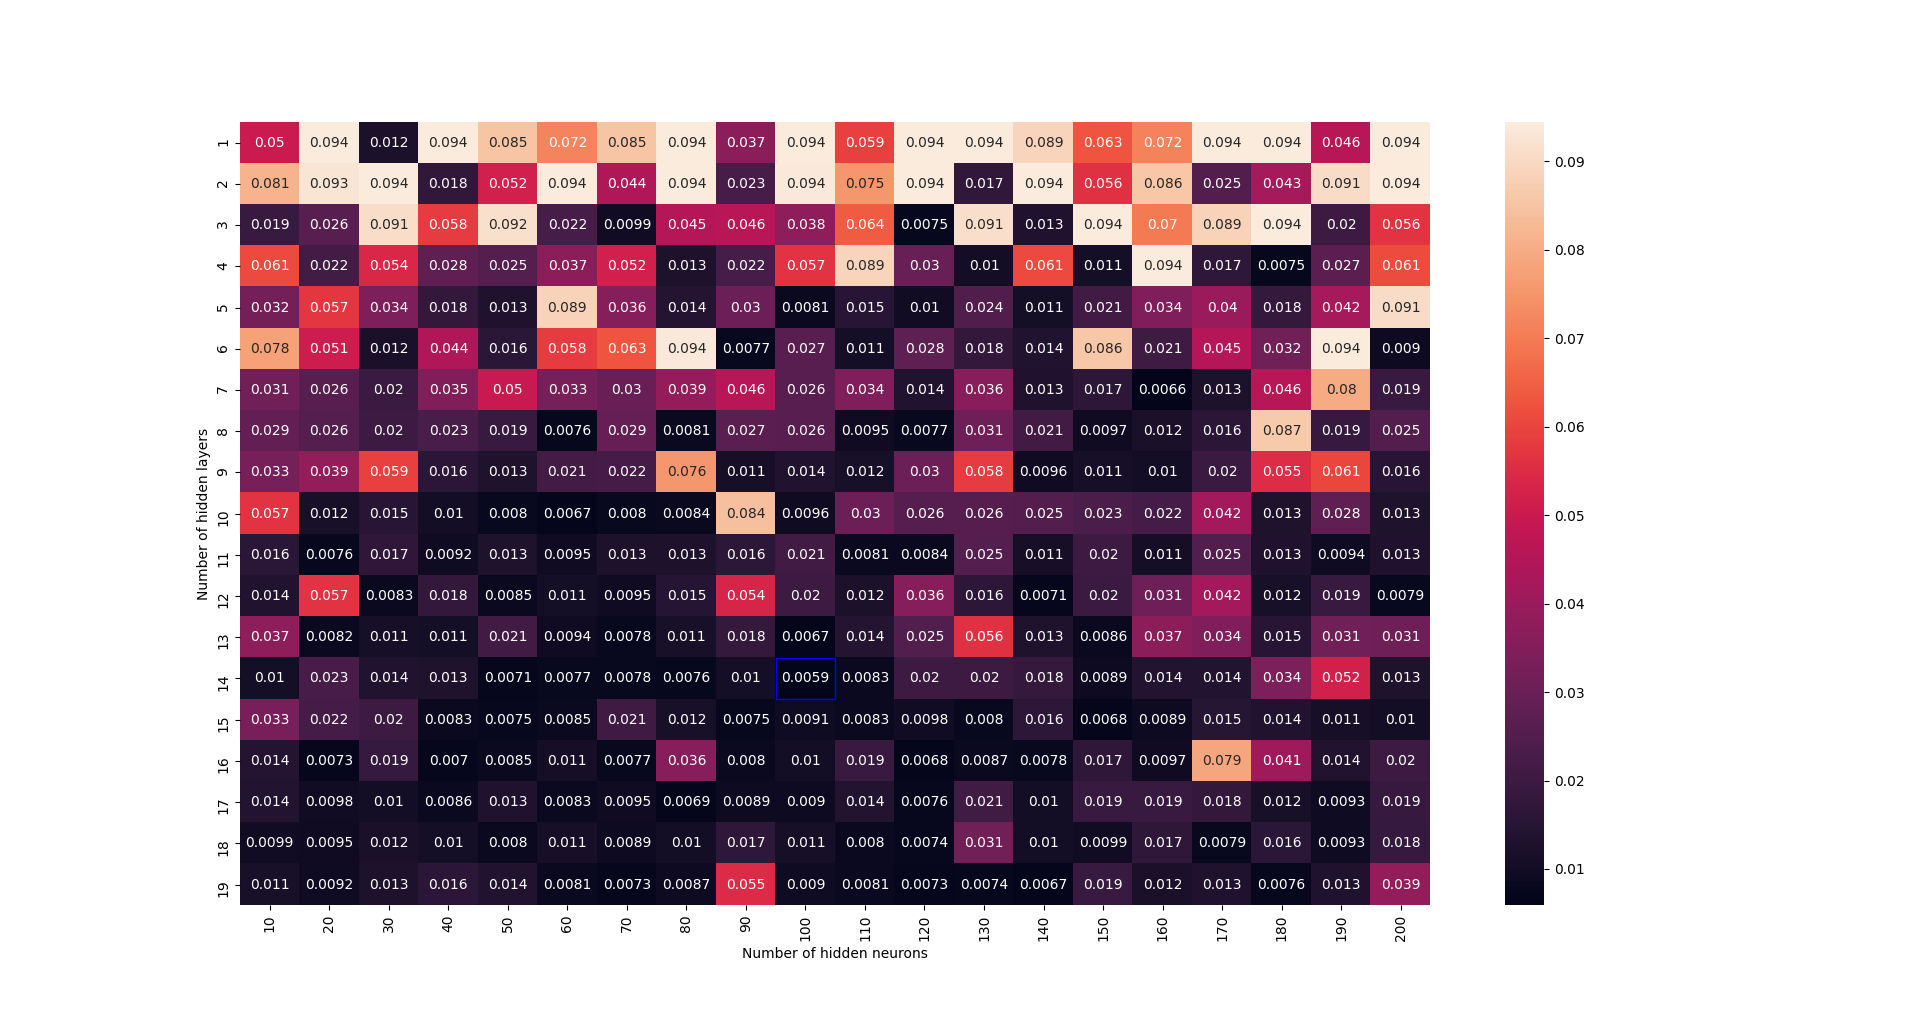
\includegraphics[width = 1\linewidth]{C:/Users/Sander/Documents/GitHub/FYS-STK4155/Project2/Project2/Report/Figures/heatmapOLS_static_mine.PNG}
\caption{\label{fig:heatOLS} Heatmap showing the MSE for my own neural network for different numbers of hidden layers and hidden neurons. Blue square at 100 neurons and 14 layers indicate the area of lowest MSE. Here we have utilized the OLS implementation.}
\end{figure}

\begin{figure}[H]
\centering
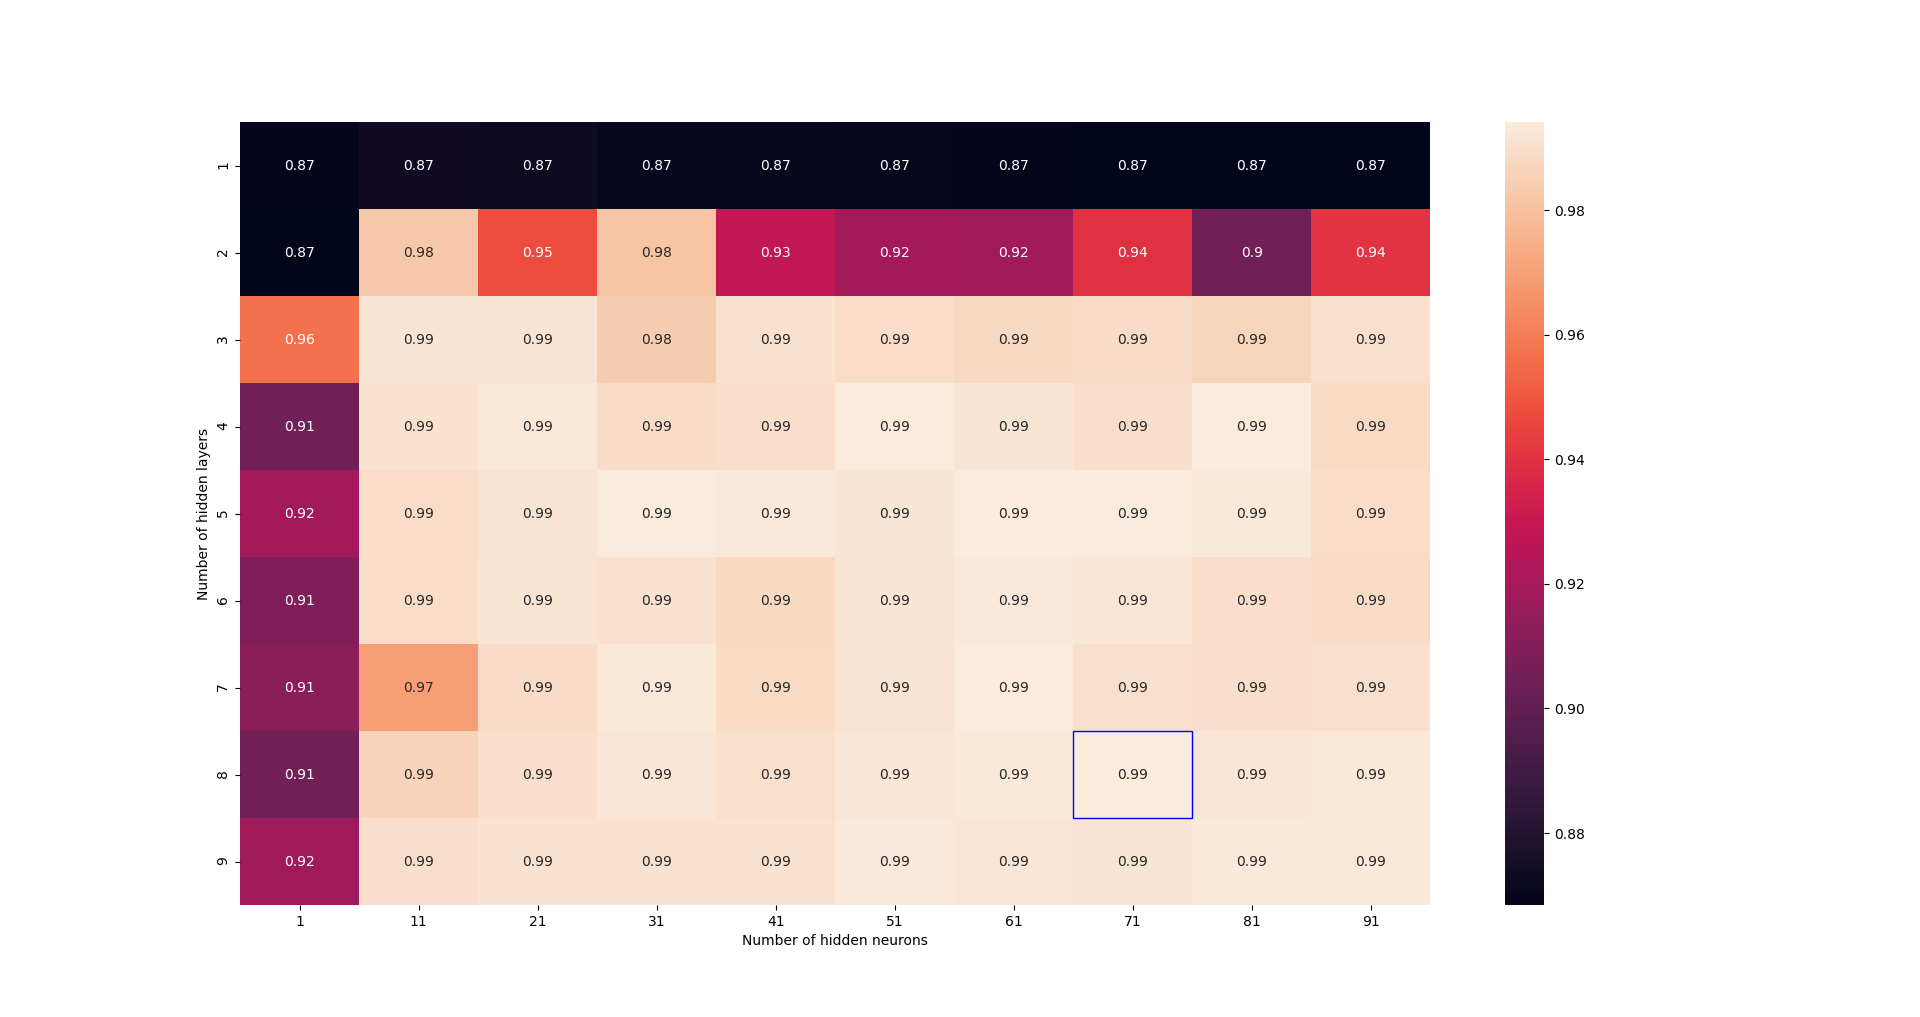
\includegraphics[width = 1\linewidth]{C:/Users/Sander/Documents/GitHub/FYS-STK4155/Project2/Project2/Report/Figures/heatmapOLS_static_mineR2.PNG}
\caption{\label{fig:heatOLSR2} Heatmap showing the $R^2$ for my own neural network for different numbers of hidden layers and hidden neurons. Blue square at 100 neurons and 14 layers indicate the area of highest $R^2$. Here we have utilized the OLS implementation.}
\end{figure}

\begin{figure}[H]
\centering
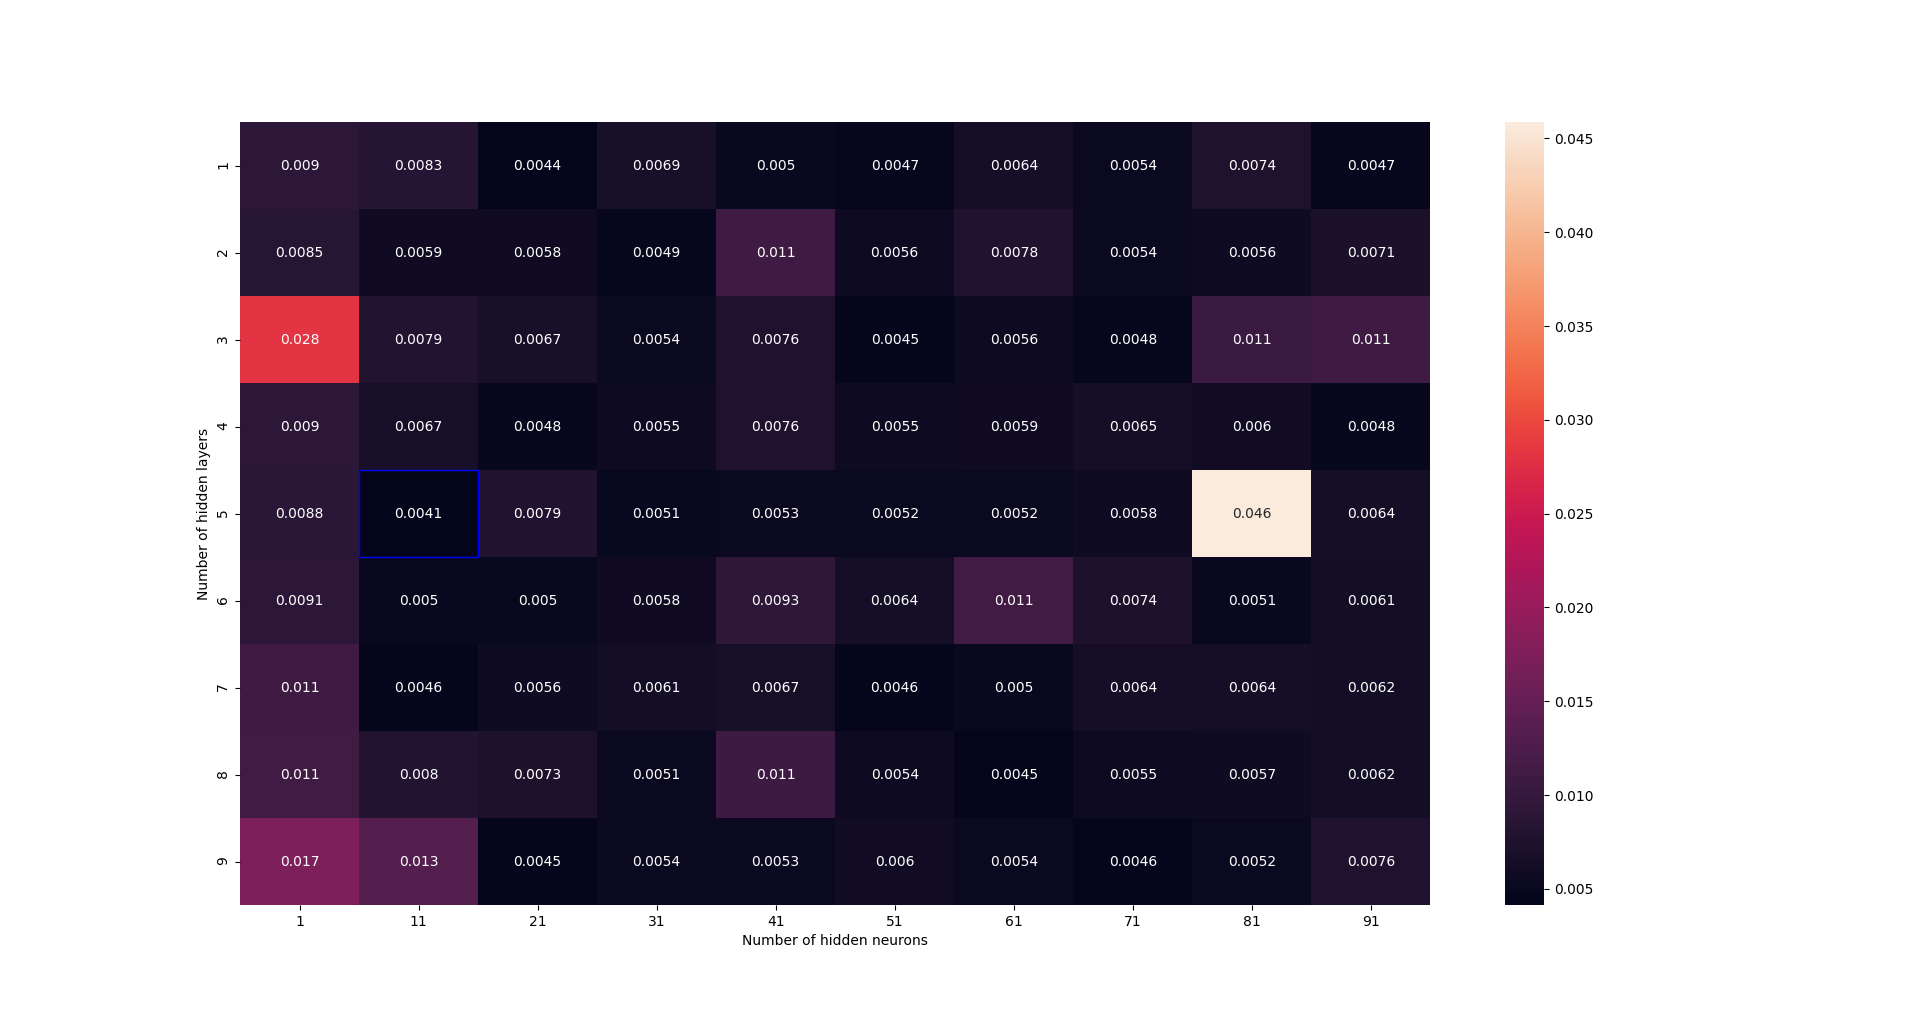
\includegraphics[width = 1\linewidth]{C:/Users/Sander/Documents/GitHub/FYS-STK4155/Project2/Project2/Report/Figures/heatmapOLS_static_scikit.PNG}
\caption{\label{fig:heatOLSsci} Heatmap showing the MSE using Scikit implementation for different numbers of hidden layers and hidden neurons. Blue square at 180 neurons and 9 layers indicate the area of lowest MSE. Here we have utilized the OLS implementation.}
\end{figure}

\begin{figure}[H]
\centering
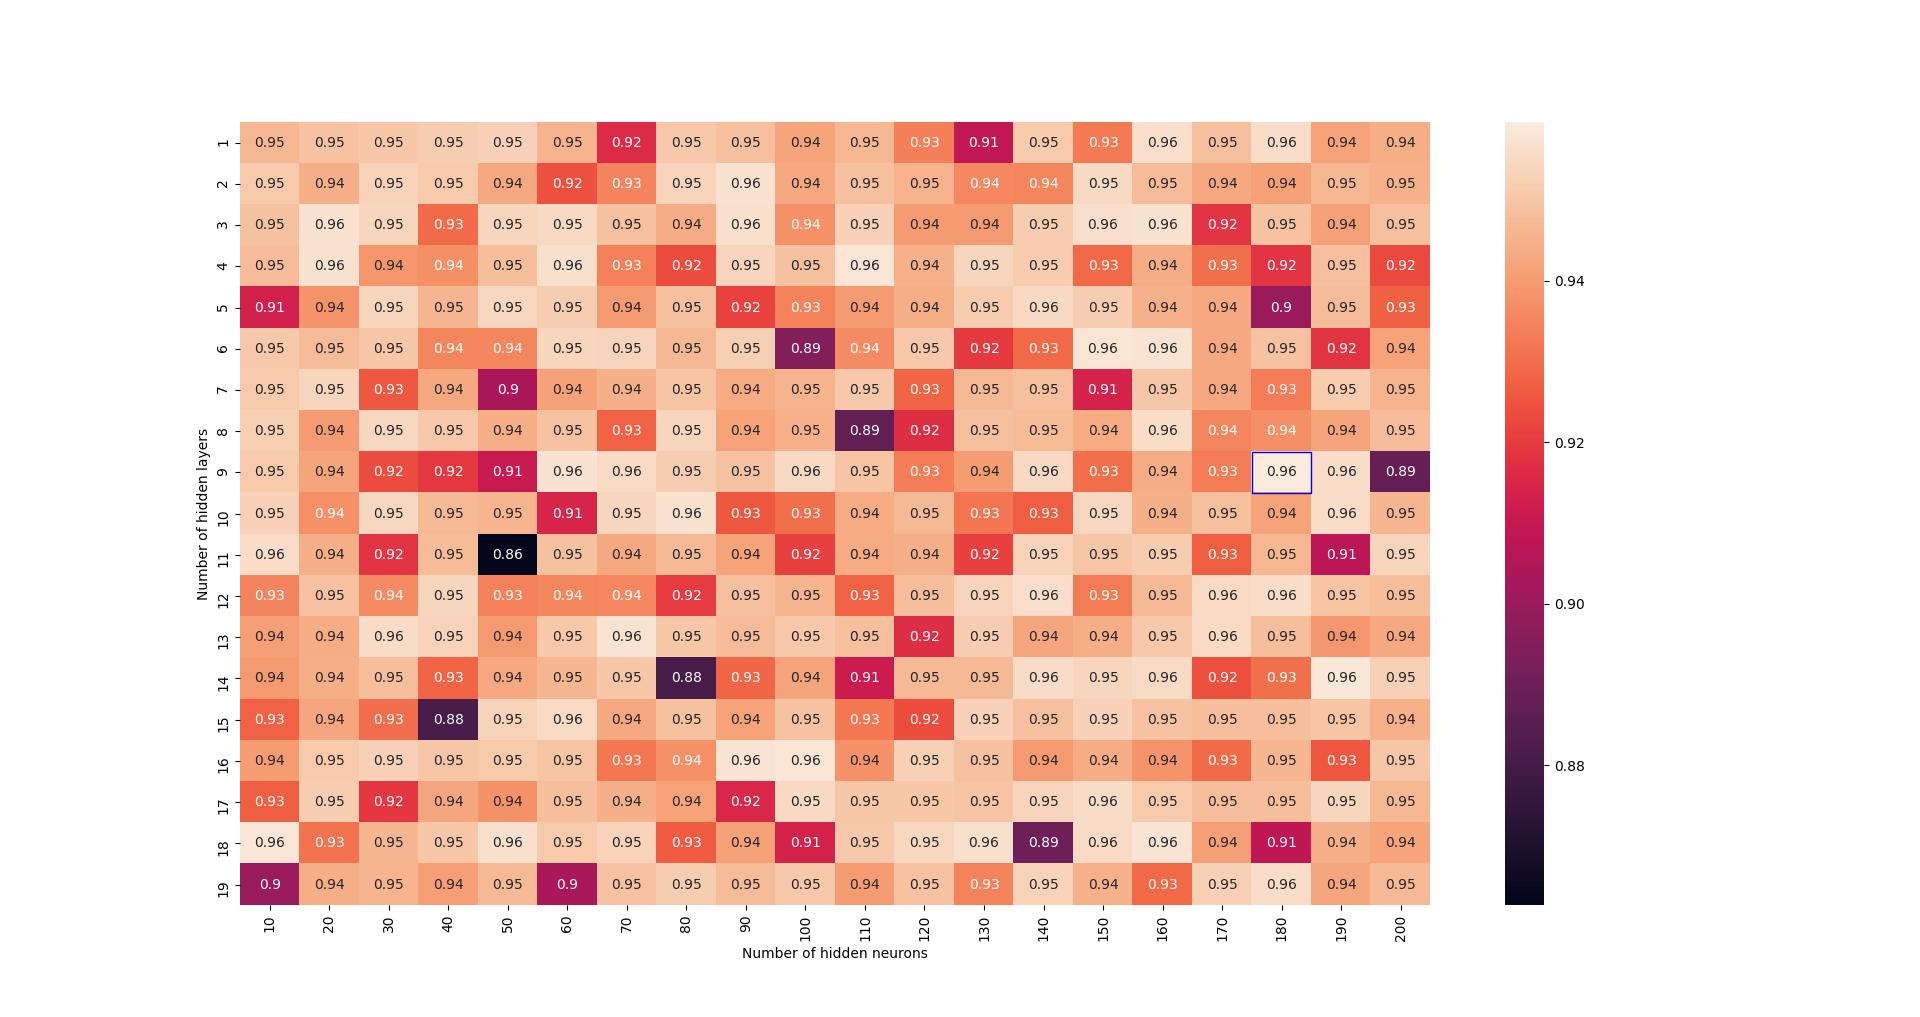
\includegraphics[width = 1\linewidth]{C:/Users/Sander/Documents/GitHub/FYS-STK4155/Project2/Project2/Report/Figures/heatmapOLS_static_scikitR2.PNG}
\caption{\label{fig:heatOLSsciR2} Heatmap showing the $R^2$ using Scikit implementation for different numbers of hidden layers and hidden neurons. Blue square at 180 neurons and 9 layers indicate the area of highest $R^2$. Here we have utilized the OLS implementation.}
\end{figure}

\begin{figure}[H]
\centering
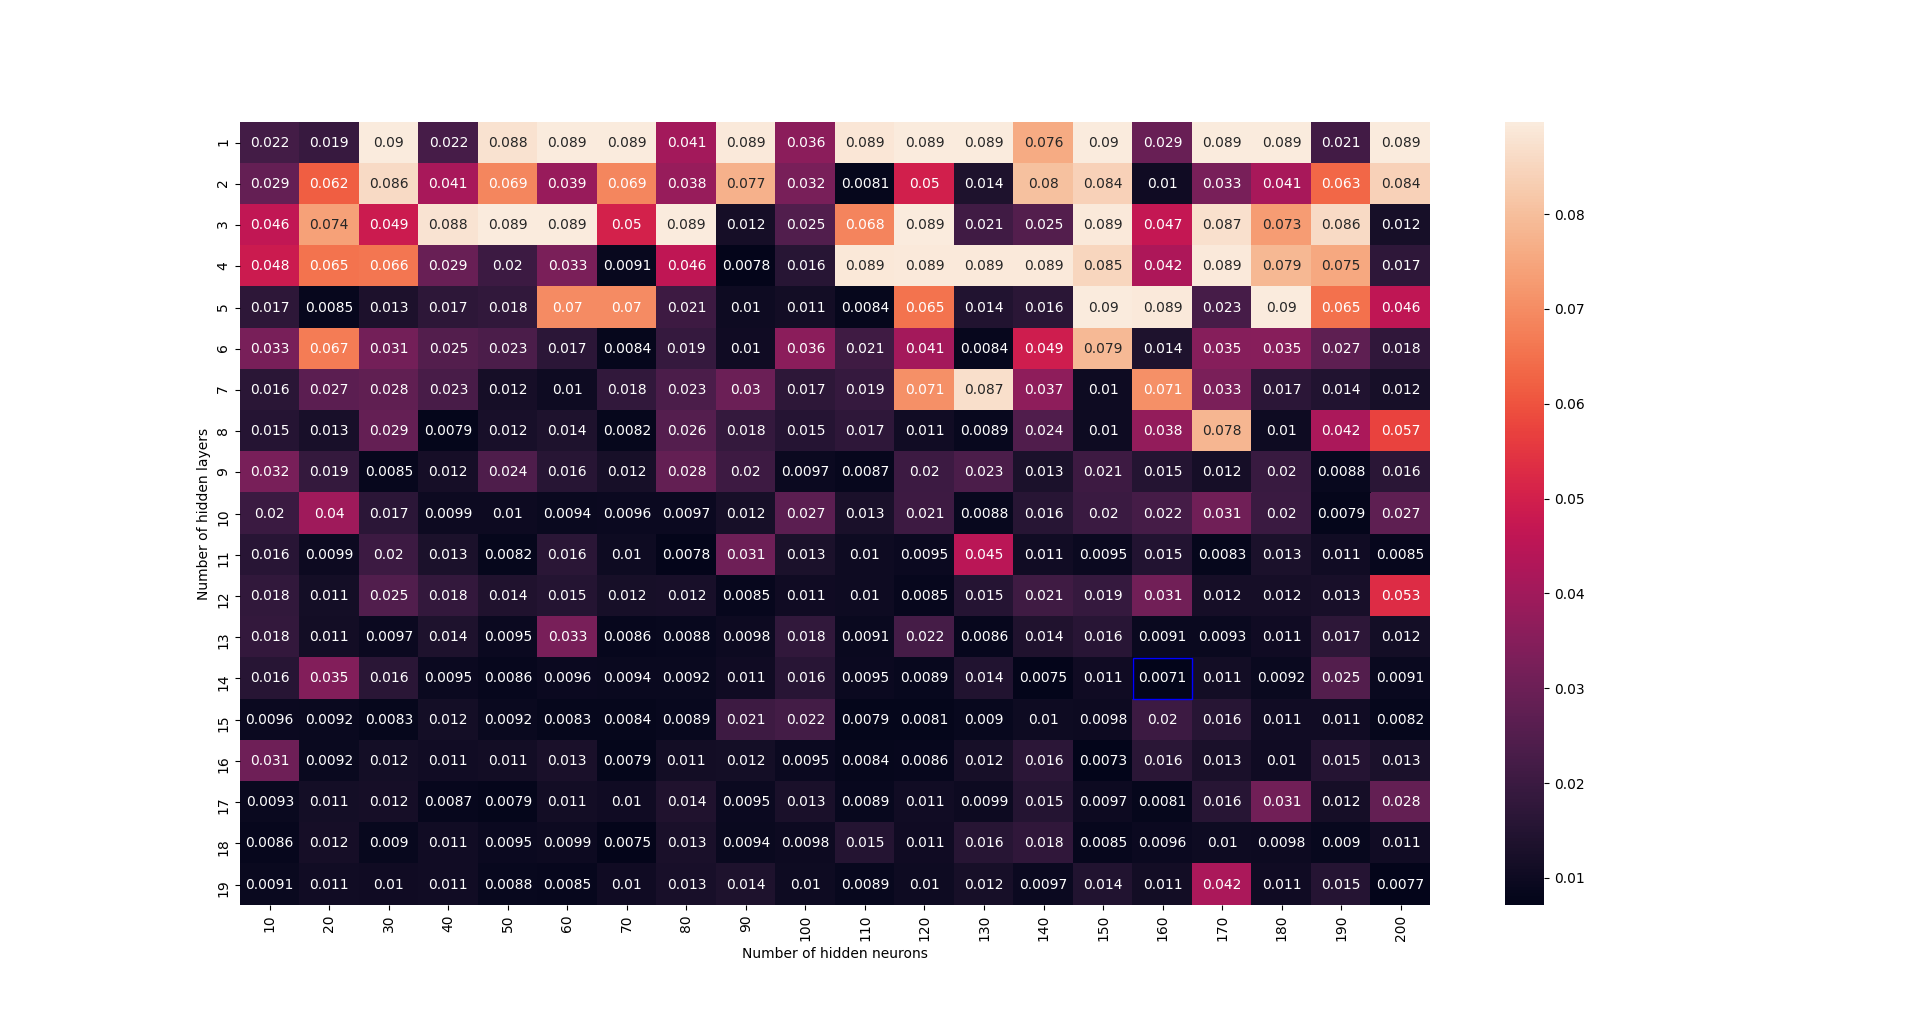
\includegraphics[width = 1\linewidth]{C:/Users/Sander/Documents/GitHub/FYS-STK4155/Project2/Project2/Report/Figures/heatmapRidge_static_mine.PNG}
\caption{\label{fig:heatRidge} Heatmap showing the MSE for my own neural network for different numbers of hidden layers and hidden neurons. Blue square at 160 neurons and 14 layers indicate the area of lowest MSE. Here we have utilized the Ridge implementation.}
\end{figure}

\begin{figure}[H]
\centering
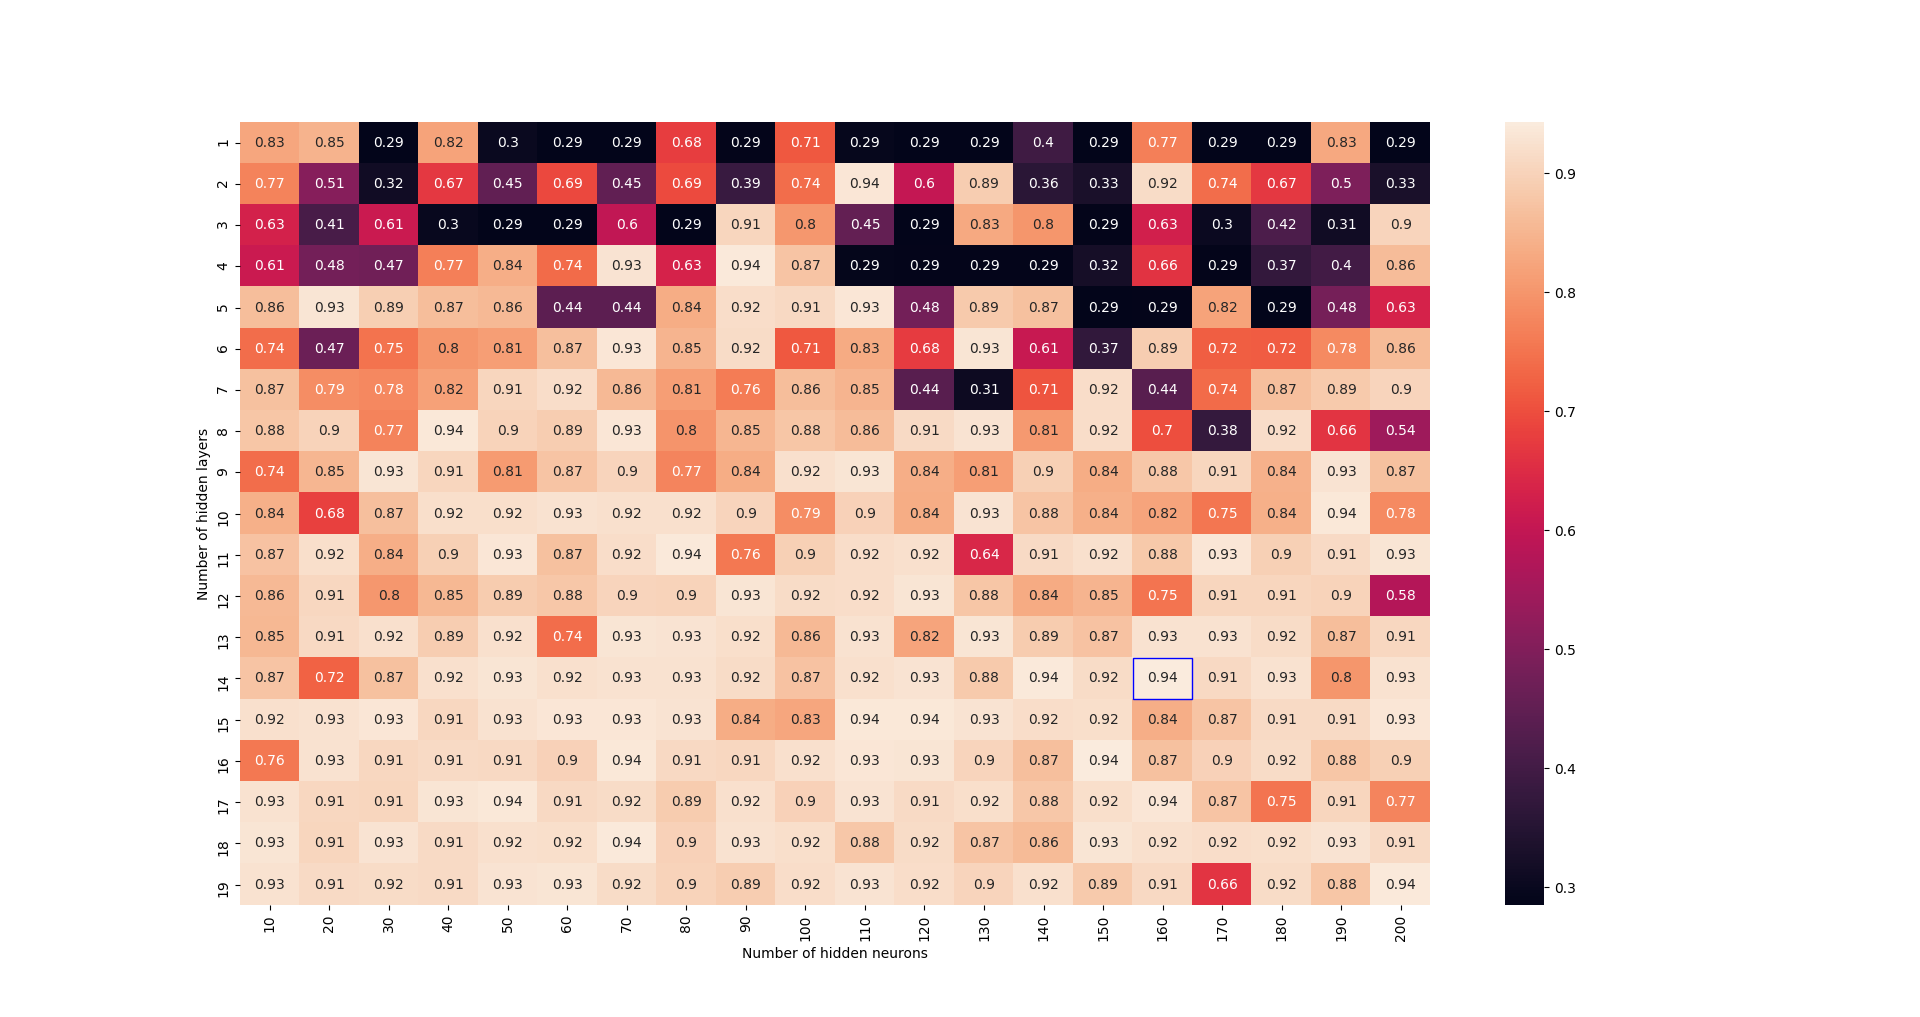
\includegraphics[width = 1\linewidth]{C:/Users/Sander/Documents/GitHub/FYS-STK4155/Project2/Project2/Report/Figures/heatmapRidge_static_mineR2.PNG}
\caption{\label{fig:heatRidgeR2} Heatmap showing the $R^2$ for my own neural network for different numbers of hidden layers and hidden neurons. Blue square at 160 neurons and 14 layers indicate the area of lowest MSE. Here we have utilized the Ridge implementation.}
\end{figure}

\begin{figure}[H]
\centering
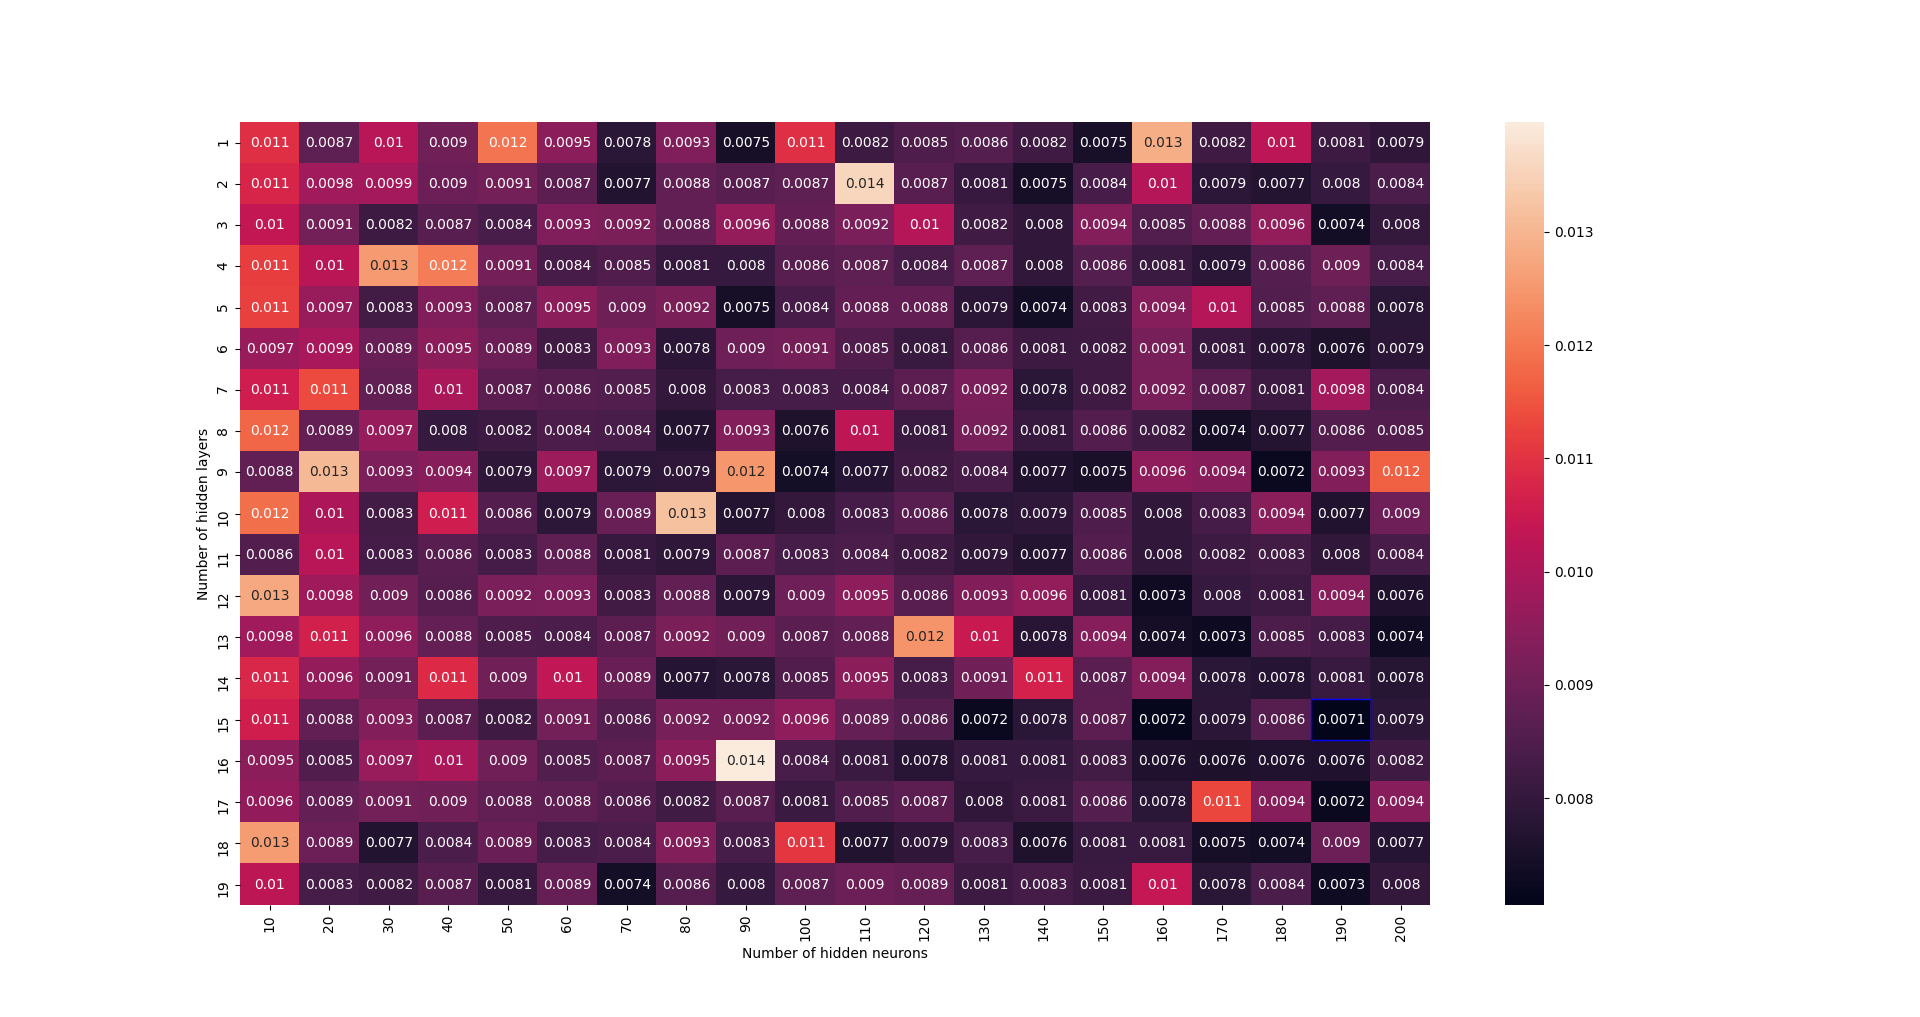
\includegraphics[width = 1\linewidth]{C:/Users/Sander/Documents/GitHub/FYS-STK4155/Project2/Project2/Report/Figures/heatmapRidge_static_scikit.PNG}
\caption{\label{fig:heatRidgesci} Heatmap showing the MSE using Scikit implementation for different numbers of hidden layers and hidden neurons. Blue square at 190 neurons and 15 layers indicate the area of lowest MSE. Here we have utilized the Ridge implementation.}
\end{figure}

\begin{figure}[H]
\centering
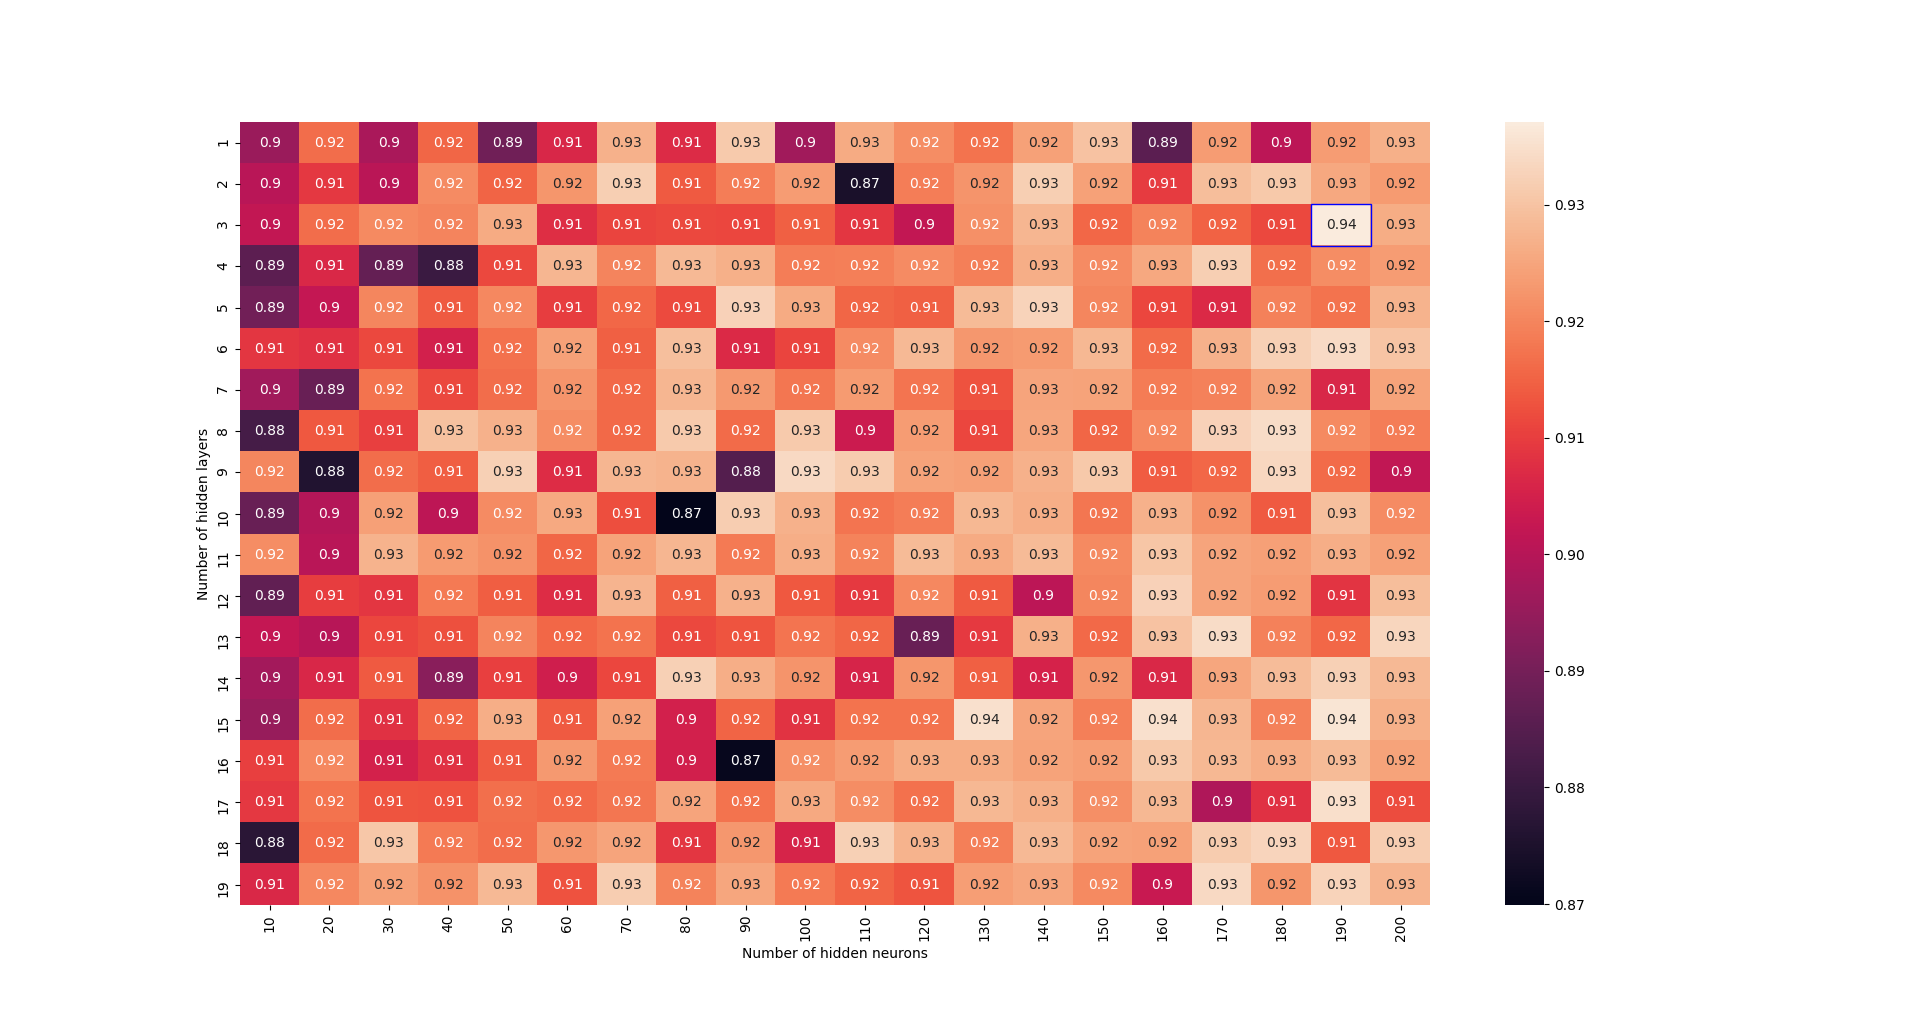
\includegraphics[width = 1\linewidth]{C:/Users/Sander/Documents/GitHub/FYS-STK4155/Project2/Project2/Report/Figures/heatmapRidge_static_scikitR2.PNG}
\caption{\label{fig:heatRidgesciR2} Heatmap showing the $R^2$ using Scikit implementation for different numbers of hidden layers and hidden neurons. Blue square at 190 neurons and 3 layers indicate the area of lowest MSE. Here we have utilized the Ridge implementation.}
\end{figure}

\noindent We first compare the OLS implementations and see that my own implementation seems to struggle quite a lot at a low number of layers, while the Scikit implementation seems to do just fine at any number of layers as seen from figures \ref{fig:heatOLS} and \ref{fig:heatOLSsci}. This is supported by looking at the $R^2$ values in figures \ref{fig:heatOLSR2} and \ref{fig:heatOLSsciR2}. However, for number of layers above 8, my own implementation is comparable to that of the Scikit as the minimum MSEs found were $0.0059$ for my own implementation and $0.0051$ for the Scikit implementation. 
\\
It is also observed that the minimum MSE is located at different values of hidden neurons and hidden layers for my own implementation and the Scikit implementation. However, seeing as the MSE does not really change that much after a $9$ or $10$ hidden layers, this is pretty meaningless. As long as we chose the number of layers to be significantly large, it seems the algorithm performs very well.
\\
The Ridge implementation seen in figure \ref{fig:heatRidge}, \ref{fig:heatRidgeR2}, \ref{fig:heatRidgesci} and \ref{fig:heatRidgesciR2} are quite interesting as the MSE seems to depend on the number of neurons as well as the number of layers. This is evident in my own implementation, but even more so in the Scikit implementation. There are very high MSE values for lower number of hidden neurons per layer, but the MSE decreases as we increase the number of hidden neurons. The size of the layer seem to be less in this case.

\newpage

\begin{center}
\Large{\textbf{Exercise 1c): Testing different activation functions}}
\end{center}

\begin{center}
\large{\textbf{The RELU activation functions}}
\end{center}

\noindent So far we have only utilized the sigmoid function in our hidden neurons as defined in equation \ref{eq:sig}. Now we want to experiment with two additional activation functions, namely the RELU and the leaky RELU defined in equation \ref{eq:RELU} and \ref{eq:leakyRELU}

\begin{equation}\label{eq:RELU}
\begin{aligned}
f(x) = 
\begin{cases}
x,& \text{if } x > 0\\
0,& \text{otherwise}
\end{cases}
\end{aligned}
\end{equation}

\begin{equation}\label{eq:leakyRELU}
\begin{aligned}
f(x) = 
\begin{cases}
x,& \text{if } x > 0\\
ax,& \text{otherwise}
\end{cases}
\end{aligned}
\end{equation}

\noindent We can see that this is close to the linear activation function where the input is simply passed through without any alterations. However, if the input is zero, then the output from a given neuron will be zero in the RELU case. The same goes for the leaky RELU case, but instead if setting the input values to zero, we set it to some small constant times the input. a in equation \ref{eq:leakyRELU} is typically in the range of $0.01$ and kind of has the same purpose as the bias in the way that it prevents the neuron from ever giving an output of zero (thereby the name "leaky"). Similar to the bias, this is done to prevent a chain of zeros to be passed through the neural network.
\\
We can now perform the same analysis as in exercise 1b), but using the RELU and leaky RELU instead of the sigmoid as our hidden layer activation function.

\begin{center}
\large{\textbf{Neural network results using RELU activation functions}}
\end{center}

\newpage

\begin{center}
\Large{\textbf{Exercise d): a}}
\end{center}

\noindent a

\newpage

\begin{center}
\Large{\textbf{Exercise 1e) a}}
\end{center}

\noindent a

\newpage

\begin{center}
\Large{\textbf{Exercise 1f) a}}
\end{center}

\noindent a

\newpage

\begin{center}
\Large{\textbf{Conclusion}}
\end{center}

\noindent a

\newpage

\begin{center}
\Large{\textbf{Future work}}
\end{center}

\noindent a

\newpage

\begin{center}
\Large{\textbf{References}}
\end{center}

\begin{itemize}
  \item a
\end{itemize}

\end{document}
